\documentclass[11pt]{article}
\usepackage[margin=1.25in]{geometry}
\usepackage{setspace}
\usepackage{fancyhdr}
\usepackage[T1]{fontenc}
\usepackage{microtype} 
\usepackage{mathpazo} %
\usepackage[utf8]{inputenc} %
\usepackage{nomencl}
\usepackage{siunitx}
\makenomenclature
\renewcommand{\nomname}{Nomenclature}


\pagestyle{fancy}
\lhead{} \chead{} \rhead{}
\lfoot{} \cfoot{\thepage} \rfoot{}
\renewcommand{\headrulewidth}{0pt}
\renewcommand{\footrulewidth}{0pt}



\setlength{\parskip}{.6\baselineskip}
\setlength{\parindent}{0pt}

\usepackage[centertags]{amsmath}
\usepackage{amssymb}
\usepackage{bm}
\usepackage[psamsfonts,mathscr]{eucal}
\usepackage[Symbol]{upgreek}
\usepackage{mathtools}
\usepackage{amsfonts}

\renewcommand{\vec}[1]{\mathbf{#1}}
\newcommand{\mat}[1]{\mathsf{#1}}
\newcommand{\tp}[1]{{#1}^{\footnotesize T}}
\setlength{\abovedisplayskip}{0pt}
\setlength{\belowdisplayskip}{0pt}
\setlength{\abovedisplayshortskip}{0pt}
\setlength{\belowdisplayshortskip}{0pt}

\usepackage{graphicx}
\graphicspath{{Figures/}}





\usepackage{afterpage}

\usepackage[table,xcdraw]{xcolor}
\usepackage{tikz}
\usepackage{wrapfig}
\definecolor{PlainBlue}{rgb}{0,0,.7}
\definecolor{PlainRed}{rgb}{.7,0,0}
\definecolor{BrownRed}{rgb}{.77,0.33,0.31}
\definecolor{ForestGreen}{HTML}{1b6f1b}



\usepackage{tikz}
\usetikzlibrary{shapes.geometric, arrows.meta, positioning}


\usepackage{multirow}
\usepackage{multicol}
\usepackage{booktabs}
\usepackage[most]{tcolorbox}
\usepackage{blindtext}
\usepackage{enumitem}
\usepackage{float}
\usepackage{stfloats}
\usepackage{afterpage}
\usepackage[normalem]{ulem}
\usepackage[export]{adjustbox}
\usepackage[labelformat=parens]{subcaption}
\usepackage{caption}
\captionsetup[figure]{labelfont={bf}}
\captionsetup[table]{labelfont={bf}}

\usepackage[numbers,sort&compress]{natbib}
\usepackage[colorlinks=true,citecolor=ForestGreen,linkcolor=BrownRed,urlcolor=PlainBlue,bookmarks=false]{hyperref}
\usepackage[capitalise]{cleveref}


\usepackage{algorithmicx}
\usepackage{algorithm}
\usepackage{algcompatible}
\usepackage{pgfplots}
\pgfplotsset{compat=1.17}

\usepackage{authblk}


\usepackage{epsfig}
\setlength{\textfloatsep}{0pt}
\setlength{\belowcaptionskip}{11pt}
\renewcommand{\topfraction}{0.9}
\renewcommand{\dbltopfraction}{0.9}
\renewcommand{\textfraction}{0.07}
\renewcommand{\floatpagefraction}{0.85}
\renewcommand{\dblfloatpagefraction}{0.9}
\setlength{\intextsep}{10pt plus 2pt minus 2pt}
\setlength{\textfloatsep}{10pt plus 2pt minus 2pt}
\renewcommand{\arraystretch}{1.7}

\renewcommand{\footnoterule}{%
	\kern -3pt
	\hrule width \textwidth height 0.5pt
	\kern 2pt%
}
\setlength{\skip\footins}{1cm}

\usepackage[colorinlistoftodos,prependcaption,textsize=tiny]{todonotes}
\usepackage{xargs}
\newcommandx{\unsure}[2][1=]{\todo[linecolor=red,backgroundcolor=red!25,bordercolor=red,#1]{#2}}
\newcommandx{\change}[2][1=]{\todo[linecolor=blue,backgroundcolor=blue!25,bordercolor=blue,#1]{#2}}
\newcommandx{\info}[2][1=]{\todo[linecolor=OliveGreen,backgroundcolor=OliveGreen!25,bordercolor=OliveGreen,#1]{#2}}
\newcommandx{\improvement}[2][1=]{\todo[linecolor=Plum,backgroundcolor=Plum!25,bordercolor=Plum,#1]{#2}}
\newcommandx{\thiswillnotshow}[2][1=]{\todo[disable,#1]{#2}}

\usepackage{nomencl}
\makenomenclature
\renewcommand{\nomname}{List of Symbols and Abbreviations}
\setlength{\nomlabelwidth}{2cm} %



\usepackage{amsthm}
\usepackage[english]{babel}
\newtheorem{theorem}{Theorem}[section]


\renewcommand{\algorithmicrequire}{\textbf{Input:}}
\renewcommand{\algorithmicensure}{\textbf{Output:}}
\newcommand{\podjac} {\ensuremath{\Phi_\jac}}
\newcommand{\podres} {\ensuremath{\Phi_\res}}

\newcounter{remarkcounter}
\setcounter{remarkcounter}{0}

\newcommand{\remark}{%
    \refstepcounter{remarkcounter} %
    \paragraph{Remark~\arabic{remarkcounter}}%
}







\title{\vspace{-2pt}{\bf Hyper-reduction Techniques for Efficient Simulation of Large-Scale Engineering Systems: A Tutorial}}

\author[1]{Suparno Bhattacharyya}
\author[1,2]{Jian Tao}%
\author[3]{Eduardo Gildin}
\author[4]{Jean Ragusa}

\affil[1]{Institute of Data Science\\Texas A\&M University, College Station, TX, USA}
\affil[2]{College of Performance, Visualization \& Fine Arts\\Texas A\&M University, College Station, TX, USA}
\affil[3]{Department of Petroleum Engineering\\Texas A\&M University, College Station, TX, USA}
\affil[4]{Department of Nuclear Engineering\\Texas A\&M University, College Station, TX, USA}

\date{}




\begin{document}

% Extracted equation environments
\begin{equation}
\left\{
\begin{array}{l}
\mat{M}(\boldsymbol{\mu})\dot{\vec{w}}(\vec{x},t; \boldsymbol{\mu}) + \vec{f}(\vec{w}(\vec{x},t; \boldsymbol{\mu}); \boldsymbol{\mu}) = \vec{g}(\vec{x},t; \boldsymbol{\mu}),\\
\vec{w}(\vec{x},0; \boldsymbol{\mu}) = \vec{w}^0(\vec{x};\boldsymbol{\mu}),
\end{array}
\right.
\label{eq:gov_eq}
\end{equation}

\begin{equation}
 \underset{ U \in L^2(\Omega)}{\operatorname{min}} \Big \langle \| w(x,t) - ( w(x,t), U(x) ) U(x) \|^{2} \Big \rangle   
\end{equation}

\begin{equation}
\mathfrak{R} U = \lambda U, \quad \mathfrak{R} U = \langle (w, U)w \rangle,
\end{equation}

\begin{equation}
r_k = \frac{\sum_{i=1}^k \lambda_i}{\sum_{i=1}^N \lambda_i}
\label{eq:mode_sel}
\end{equation}

\begin{equation}
\epsilon_{\text{POD}} = \sqrt{\sum_{i=k+1}^N \lambda_i}
\end{equation}

\begin{equation}
	\mat{W}=\left[\begin{array}{cccc}
	\mathbf{w}_{1} - \mathbf{w}^{ref} & \mathbf{w}_{2} - \mathbf{w}^{ref}& \cdots & \mathbf{w}_{N_t} - \mathbf{w}^{ref}\\
	\end{array}\right]
\label{eq:data_W}
\end{equation}

\begin{equation}
\mat{R} = \frac{1}{N_t}\mat{W}\mat{W}^\top
\label{eq:cor_mat}
\end{equation}

\begin{equation}
\frac{1}{N_t}\mat{W}^\top\mat{W}\vec{q} = \lambda\vec{q}, \quad \mathbb{U} = \mat{W}\vec{q}
\end{equation}

\begin{equation}
\mat{W} = \underline{\mathbb{U}}\mat{\Sigma}\underline{\mathbb{V}}^\top
\label{eq:svd}
\end{equation}

\begin{equation}
\mat{R} = \frac{1}{N_t} \underline{\mathbb{U}} \mat{\Sigma} \mat{\Sigma}^\top \underline{\mathbb{U}}^\top = \underline{\mathbb{U}}\mat{\Lambda}\underline{\mathbb{U}}^\top
\label{eq:pod-svd}
\end{equation}

\begin{equation}
\frac{\sigma_i^2}{N_t} = \lambda_{\text{POD}_i}
\label{eq:SVD_POD}
\end{equation}

\begin{equation}
\widetilde{\mathbb{U}} = \mathbb{U}[:,1:n]
\label{eq:U_tilde}
\end{equation}

\begin{equation}
\vec{w}_N(\vec{x},t; \boldsymbol{\mu}) \approx \widetilde{\vec{w}}_N(\vec{x},t; \boldsymbol{\mu}) = \vec{w}^{ref}_N+\widetilde{\mathbb{U}}  \vec{w}_n(\vec{x},t; \boldsymbol{\mu}),
\label{eq:w_ned_gal}
\end{equation}

\begin{equation}
\vec{r}_{N}(\vec{w}_n;\boldsymbol{\mu}) = \mat{M}(\boldsymbol{\mu})\widetilde{\mathbb{U}}\dot{\vec{w}}_n(\vec{x},t; \boldsymbol{\mu}) + \vec{f}_N(\vec{w}^{ref}_N+\widetilde{\mathbb{U}}\vec{w}_n(\vec{x},t; \boldsymbol{\mu}); \boldsymbol{\mu}) - \vec{g}_N(\vec{x},t; \boldsymbol{\mu})
\label{eq:residual_gov_eq_gal}
\end{equation}

\begin{equation}
\mathbb{W}^\top \left[ \mat{M}(\boldsymbol{\mu}) \widetilde{\mathbb{U}} \dot{\vec{w}}_n + \vec{f}_N(\vec{w}^{ref}_N+\widetilde{\mathbb{U}} \vec{w}_n; \boldsymbol{\mu}) - \vec{g}_N \right] = 0.
\label{eq:PG_projection}
\end{equation}

\begin{equation}
\mat{M}_{n}(\boldsymbol{\mu}) = \mathbb{W}^\top \mat{M}_{N}(\boldsymbol{\mu}) \widetilde{\mathbb{U}},
\end{equation}

\begin{equation}
\vec{f}_n(\vec{w}; \boldsymbol{\mu}) = \mathbb{W}^\top \vec{f}_N(\vec{w}^{ref}_N+\widetilde{\mathbb{U}} \vec{w}_n; \boldsymbol{\mu}),
\end{equation}

\begin{equation}
\vec{g}_n = \mathbb{W}^\top \vec{g}_N,
\end{equation}

\begin{equation}
\left\{
\begin{array}{l}
\mat{M}_n(\boldsymbol{\mu}) \dot{\vec{w}}_n + \vec{f}_n(\vec{w}_n; \boldsymbol{\mu}) = \vec{g}_n,\\
\vec{w}_n(\vec{x},0, \boldsymbol{\mu}) = (\mathbb{W}^\top \widetilde{\mathbb{U}})^{-1}\mathbb{W}^\top (\vec{w}_N^0(\boldsymbol{\mu})-\vec{w}^{ref}_N)
\end{array}
\right.
\label{eq:ROM_eq}
\end{equation}

\begin{equation}
-\nabla \cdot (k \nabla T) = q \quad \text{in} \quad \Omega,
\label{eq:heat_pde}
\end{equation}

\begin{equation}
   \left. g\right|_{x = 0} = 0\, \unit{W} \quad \text{and} \quad \left.T\right|_{x = 0.5} = 573.15 \, \text{K} 
\end{equation}

\begin{equation}
\int_{\Omega} k(T;\boldsymbol\mu)\nabla T \cdot \nabla v \, d\Omega  = \int_{\Omega} q v \, d\Omega 
\label{eq:weak_pde}
\end{equation}

\begin{equation}
\widehat{T}(x) \approx \sum_{i=1}^{N} T_i \phi_i(x),
\label{eq:FE_shape}
\end{equation}

\begin{equation}
\mat{K}_N(\vec{T}_N;\boldsymbol\mu) \vec{T}_N = \vec{f}_N
\label{eq:HC_HDM}
\end{equation}

\begin{equation}
\mat{K}_N(\mathbf{T}_N; \boldsymbol\mu) = \sum_{e=1}^{n_{\text{cell}}} \mat{Q}_e^\top \mat{K}^e (\mat{Q}_e\mathbf{T}_N; \boldsymbol\mu) \mat{Q}_e,
\label{eq:elemental_contrib_K}
\end{equation}

\begin{equation}
\mathbf{f}_N = \sum_{e=1}^{n_{\text{cell}}} \mat{Q}_e^\top \vec{f}^e_{d_e}(\boldsymbol\mu),
\label{eq:elemental_contrib_f}
\end{equation}

\begin{equation}
\mat{K}^e_{ij} = \int_{\Omega^{e}} k\left(\sum_{s=1}^{d_e} T_s \phi^e_s;\boldsymbol\mu\right) \nabla \phi^e_i \cdot \nabla \phi^e_j \, d\Omega^{e}
\label{eq:K_N_ij}
\end{equation}

\begin{equation}
{f}^e_i = \int_{{\Omega}^e} q \phi_i \, d\Omega^{e}.
\label{eq:f_N_ij}
\end{equation}

\begin{equation}
k(\mu) = 
\begin{cases} 
k_1 = \mu + 16, & \text{for} \quad 0.0 \leq x < 0.4   \\ 
k_2 = \mu + 30, & \text{for} \quad 0.4 \leq x \leq 0.5   
\end{cases}
\label{eq:k_mu_L}
\end{equation}

\begin{equation}
k(T,\mu) = 
\begin{cases} 
k_1 =\mu + 16 + 2150/(T - 73.15),  &\quad 0.0 \leq x < 0.4 \\ 
k_1 =\mu + 30 + 2.09 \times 10^{-2} T - 1.45 \times 10^{-5} T^2 + 7.67 \times 10^{-9} T^3, & \quad 0.4 \leq x \leq 0.5 
\end{cases}
\label{eq:k_mu_NL}
\end{equation}

\begin{equation}
q= 
\begin{cases} 
q_1(\beta) = \beta + 35000, & \text{linear, for} \quad 0.0 \leq x < 0.4 \\ 
q_1(T,\beta) = \beta + 35000 + T/10, & \text{nonlinear, for} \quad 0.0 \leq x < 0.4 \\ 
q_2(\beta) = 10\beta + 5000 & \text{(both) for} \quad 0.4 \leq x \leq 0.5 
\end{cases}
\label{eq:q_beta}
\end{equation}

\begin{equation}
\widehat{\vec{T}}_N = \overline{\vec{T}}_N + \mathbb{\widetilde{U}} \vec{T}_n
\label{eq:T_rec}
\end{equation}

\begin{equation}
\mat{K}_n\vec{T}_n = \vec{f}_n- \widetilde{\mathbb{U}}^\top \mat{K}_N\overline{\vec{T}}_N 
\label{eq:HC_ROM}
\end{equation}

\begin{equation}
e_T = 100\times\dfrac{\|\vec{T}_{N}(\mu,\beta)_k-\widehat{\vec{T}}_N(\mu,\beta)_k\|_2}{\|\vec{T}_{N}(\mu,\beta)_k\|_2}
\label{eq:rom_error}
\end{equation}

\begin{equation}
r_s = \dfrac{t_{HFM}}{t_{ROM}}
\label{eq:rom_speedup}
\end{equation}

\begin{equation}
\mathbf{f}_N = \mat{K} \mathbf{w}_N + \mat{B} (\mathbf{w}_N \otimes \mathbf{w}_N) + \mat{C} (\mathbf{w}_N \otimes \mathbf{w}_N \otimes \mathbf{w}_N) + \dots
\label{eq:poly_non}
\end{equation}

\begin{equation}
\mathbf{w}_N \otimes \mathbf{w}_N = [w_1^2, w_1w_2, \dots, w_1w_n, w_2w_1, w_2^2, \dots, w_2w_n, \dots, w_n^2] \in \mathbb{R}^{N^2}.
\label{eq:op}
\end{equation}

\begin{equation}
\widetilde{\mathbb{U}}^\top\vec{f}_N = \mathbf{f}_n =  \mat{K}_n \mathbf{w}_n + \mat{B}_n (\mathbf{w}_n \otimes \mathbf{w}_n) + \mat{C}_n (\mathbf{w}_n \otimes \mathbf{w}_n \otimes \mathbf{w}_n) + \dots
\label{eq:red_poly_non}
\end{equation}

\begin{equation}
\mat{K}_n = \widetilde{\mathbb{U}}^\top \mat{K} \widetilde{\mathbb{U}}, \quad \mat{B}_n = \widetilde{\mathbb{U}}^\top \mat{B} (\widetilde{\mathbb{U}} \odot \widetilde{\mathbb{U}}), \quad \mat{C}_n = \widetilde{\mathbb{U}}^\top \mat{C} (\widetilde{\mathbb{U}} \odot \widetilde{\mathbb{U}} \odot \widetilde{\mathbb{U}}),
\label{eq:red_matrices}
\end{equation}

\begin{equation}
\widetilde{\mathbb{U}} \odot \widetilde{\mathbb{U}} = [\mathbf{U}_1 \otimes \mathbf{U}_1 \quad \mathbf{U}_2 \otimes \mathbf{U}_2 \quad \ldots \quad \mathbf{U}_n \otimes \mathbf{U}_n] \in \mathcal{R}^{N^2 \times n}.
\end{equation}

\begin{equation}
{\vec{w}}_r = \mat{Z}^{\top} \vec{w}_N
\end{equation}

\begin{equation}
\mat{Z} =  
\begin{pmatrix}
1 & 0 & \cdots & 0\\
0 &  \vdots & \cdots &  \vdots \\
\vdots &  0 & \cdots &  1 \\
0 &  1 & 0 &  0 \\
\end{pmatrix}
\end{equation}

\begin{equation}
\widetilde{\vec{w}}_N = \widetilde{\mathbb{U}}_f\vec{w}_n
\label{eq:rec_imag}
\end{equation}

\begin{equation}
{\vec{w}}_r \approx \mat{Z}^{\top}\widetilde{\mathbb{U}}_f\vec{w}_n
\end{equation}

\begin{equation}
   \vec{w}_n = \arg\min_{\vec{w}_n} \| \vec{w}_r - \mat{Z}^{\top}\widetilde{\mathbb{U}}_f\vec{w}_n \|_2
   \label{eq:sampling_optimization}
\end{equation}

\begin{equation}
 {\vec{w}_n} = \left(\mat{Z}^{\top}\widetilde{\mathbb{U}}_f\right)^{\dagger}\vec{w}_r = \Omega^{-1}\mat{Z}^{\top}\widetilde{\mathbb{U}}_f\vec{w}_r
\label{eq:solution_ak}
\end{equation}

\begin{equation}
    \widehat{\vec{f}}_N(\vec{w}^{\boldsymbol{\mu}}; \boldsymbol{\mu}) = \widetilde{\mathbb{U}}_f \left(\mat{Z}^\top \widetilde{\mathbb{U}}_f\right)^{\dagger} \mat{Z}^\top \vec{f}_N(\vec{w}^{\boldsymbol{\mu}}; \boldsymbol{\mu}) = \mat{M}_D \vec{f}_N(\vec{w}^{\boldsymbol{\mu}}; \boldsymbol{\mu})
    \label{eq:deim_approx}
\end{equation}

\begin{equation}
 M_D = \widetilde{\mathbb{U}}_f \left(\mat{Z}^\top \widetilde{\mathbb{U}}_f\right)^{\dagger} \mat{Z}^\top
 \label{eq:deim_mat}
\end{equation}

\begin{equation}
    \widehat{\vec{f}}_n  = \widetilde{\mathbb{U}}^\top \, \widehat{\vec{f}}_N
    \label{eq:deim_approx_fn}
\end{equation}

\begin{equation}
\mat{F} = \left[ \vec{f}_N(\vec{w}^{\boldsymbol{\mu}_1}; \boldsymbol{\mu}_1), \cdots, \vec{f}_N(\vec{w}^{\boldsymbol{\mu}_{N_s}}; \boldsymbol{\mu}_{N_s}) \right] \approx \widetilde{\mathbb{U}}_f \mat{\Sigma}_f \mathbb{V}_f^\top.
\end{equation}

\begin{equation}
    \|\vec{f}_N - \widehat{\vec{f}}_N\|_2 \le \|\left(\mat{Z}^\top \widetilde{\mathbb{U}}_f\right)^{\dagger}\|_2 \, \| (\mat{I}-\widetilde{\mathbb{U}}_f\widetilde{\mathbb{U}}_f^{\top})\vec{f}_N\|_2
    \label{eq:deim_error}
\end{equation}

\begin{equation}
\left(\mat{Z}^{\top}\widetilde{\mathbb{U}}_f\right)^{\dagger} = \Omega^{-1}\mat{Z}^{\top}\widetilde{\mathbb{U}}_f
\label{eq:sopt_error}
\end{equation}

\begin{equation}
    \mathscr{S}(\mat{P}) = \left( \frac{\sqrt{|\det \left( \mat{P}^\top \mat{P}\right)}|} {\Pi_{i=1}^r \|\mat{P}[:,i]\|}\right)^{\frac{1}{r}}
\end{equation}

\begin{equation}
\mat{Z}^*_{\text{S-OPT}} = \underset{\mat{Z}  \in \mathbb{R}^{N \times n}}{\arg\max} \, \mathscr{S}(\mat{Z}^\top \mat{Q})
\label{eq:sopt_max}
\end{equation}

\begin{equation} 
|\det(\mat{M})| \leq \prod_{i=1}^{p} M_{ii}, 
\end{equation}

\begin{equation}
\vec{r}^{k+1}_{N} = \mat{M}(\boldsymbol{\mu})\widetilde{\mathbb{U}}\left(\vec{w}^{k+1}_n-\vec{w}^{k}_n\right) + \Delta t\,\vec{f}^{k+1}_N(\vec{w}^{ref} + \widetilde{\mathbb{U}}\vec{w}^{k+1}_n,\mu) -  \Delta t\,\vec{g}^{k+1}_N
\end{equation}

\begin{equation}
\vec{w}^{k+1}_n = \arg\min_{\mathbf{w}^{k+1}_n} \|\mathbf{r}_N^{k+1}(\vec{w}^{k+1}_n)\|_2
\label{eq:res_min}
\end{equation}

\begin{equation}
\phi(\mathbf{z}) = \frac{1}{2} \|\mathbf{r}(\mathbf{z})\|_2^2 = \mathbf{r}(\mathbf{z})^{\top} \mathbf{r}(\vec{z})
\label{eq:gnat_opt}
\end{equation}

\begin{equation}
\nabla\phi(\vec{z})=\mat{J}^{\top}(\vec{z})\vec{r}(\vec{z}) = 0
\label{eq:Jacobian_res}
\end{equation}

\begin{equation}
\mat{J} = \dfrac{\partial\vec{r}}{\partial \vec{z}} = \left(\mat{M}(\boldsymbol{\mu}) + \Delta t\,\mat{J}^{k+1}_{\vec{f}}\right)\widetilde{\mathbb{U}} 
\label{eq:jacobian}
\end{equation}

\begin{equation}
\vec{z}_{j+1} = \vec{z}_{j} + \boldsymbol{\Delta}_{j+1}
\label{eq:GaussNewton_app}
\end{equation}

\begin{equation}
\nabla^2\phi(\vec{z}_j)\boldsymbol{\Delta}_{j+1} = -\nabla\phi(\vec{z}_j)
\label{eq:Gauss_newton_step}
\end{equation}

\begin{equation}
\nabla^2\phi(\vec{z}_j) = \mat{J}(\vec{z})^{\top}\,\mat{J}(\vec{z})+ \sum_{i=1}^{N} \frac{\partial^2 r_i(\mathbf{z})}{\partial \mathbf{z}^2} r_i(\mathbf{z})
\label{eq:Gauss_newton_step}
\end{equation}

\begin{equation}
\mat{J}(\mathbf{z}_{j})^{\top} \mat{J}(\mathbf{z}_{j}) \boldsymbol{\Delta}_{j+1} = -\mat{J}(\mathbf{z}_{j})^{\top} \mathbf{r}(\mathbf{z}_{j})
\label{eq:normal_J}
\end{equation}

\begin{equation}
\boldsymbol{\Delta}_{j+1} = - \mat{R}^{-1}(\vec{z}_j)\mat{Q}(\vec{z}_j)\mathbf{r}(\mathbf{z}_{j})
\label{eq:normal_J2}
\end{equation}

\begin{equation}
    \boldsymbol{\Delta}_{j+1} = \arg\min_{\vec{q}}\| \mat{J}(\vec{z}_j)\vec{q} + \vec{r}(\vec{z}_j)  \|_2
    \label{eq:normal_optimization}
\end{equation}

\begin{equation}
\widetilde{\vec{r}}(\vec{z}_j) = \arg\min_{\vec{x}} \| \mat{Z}^\top \vec{r}(\vec{z}_j) - \mat{Z}^\top \widetilde{\mathbb{U}}_R \vec{x} \|_2
\end{equation}

\begin{equation}
\widetilde{\mat{J}}(\vec{z}_j) = \arg\min_{\mat{X}} \| \mat{Z}^\top {\mat{J}}(\vec{z}_j) - \mat{Z}^\top \widetilde{\mathbb{U}}_J \mat{X} \|_F
\end{equation}

\begin{equation}
\widetilde{\vec{r}}(\vec{z}_j) = \widetilde{\mathbb{U}}_R \left(\mat{Z}^\top \widetilde{\mathbb{U}}_R\right)^\dagger \mat{Z}^\top{\vec{r}}(\vec{z}_j),
\end{equation}

\begin{equation}
\widetilde{\mat{J}}(\vec{z}_j) = \widetilde{\mathbb{U}}_J \left(\mat{Z}^\top \widetilde{\mathbb{U}}_J\right)^\dagger \mat{Z}^\top{\mat{J}}(\vec{z}_j)
\end{equation}

\begin{equation}
  \tilde{\boldsymbol{\Delta}}_{j+1} = \arg\min_{\vec{q}} \| \mathscr{P} {\mat{J}}(\vec{z}_j) \vec{q} + \mathscr{Q} {\vec{r}}(\vec{z}_j) \|_2,  
\end{equation}

\begin{equation}
\tilde{\boldsymbol{\Delta}}_{j+1} = - \widetilde{\mat{R}}^{-1}(\vec{z}_j) \widetilde{\mat{Q}}(\vec{z}_j) \widetilde{\mathbb{U}}^\top_J \widetilde{\vec{r}}(\vec{z}_j)
\label{eq:normal_J2}
\end{equation}

\begin{equation}
\vec{b}_n(\vec{w}_n; \mu) \approx \widehat{\vec{b}}_n = \sum_{e=1}^{n_{\text{cell}}} \mathbb{W}_e^{\top} \vec{b}_{e} (\mathcal{Q}_e\vec{w}^{ref} + \widetilde{\mathbb{U}}_e \vec{w}_n; \mu)
\label{eq:r_n}
\end{equation}

\begin{equation}
\vec{b}_{e} (\mathcal{Q}_e\vec{w}^{ref} + \widetilde{\mathbb{U}}_e \vec{w}_n; \mu) = \vec{f}_{n,e}(\mathcal{Q}_e\vec{w}^{ref} + \widetilde{\mathbb{U}}_e \vec{w}_n; \mu) - \vec{g}_{n,e}(t; \mu) 
\label{eq:r_e}
\end{equation}

\begin{equation}
\mathbb{W}_e = \mat{Q}_e\mathbb{W}
\end{equation}

\begin{equation}
\widetilde{\mathbb{U}}_e = \mathcal{Q}_e\widetilde{\mathbb{U}}
\end{equation}

\begin{equation}
\vec{b}_n(\vec{w}_n; \mu) \approx \sum_{e\,\in\,\{1,...,n_{\text{cell}}\}} \xi_e \mathbb{W}_e^{\top} \vec{b}_e (\mathcal{Q}_e\vec{w}^{ref} + \widetilde{\mathbb{U}}_e\vec{w}_n; \mu)
\label{eq:r_n_approx}
\end{equation}

\begin{equation}
\vec{w}_n(\mu_k, t_k) = \widetilde{\mathbb{U}}^{\top} \left(\vec{w}_N(\mu_k, t_k)-\vec{w}^{ref}\right).    
\end{equation}

\begin{equation}
\vec{b}_n^{k} = \bar{\mat{G}}^{k}\, \vec{1},
\label{eq:bn_G1}
\end{equation}

\begin{equation}
\bar{\mat{G}}^k = \left[ \boldsymbol{\gamma}_n^{k,1},\ \boldsymbol{\gamma}_n^{k,2},\ \dots,\ \boldsymbol{\gamma}_n^{k,n_{\text{cell}}} \right],
\end{equation}

\begin{equation}
\vec{1} = \left[ 1,\ 1,\ \dots,\ 1 \right]^{\top}.
\end{equation}

\begin{equation}
\boldsymbol{\Gamma} = \mat{G}\, \vec{1},
\label{eq:Gamma_G1}
\end{equation}

\begin{equation}
\boldsymbol{\Gamma} = \left[ \vec{b}_n^{1\,\top}, \vec{b}_n^{2\,\top}, \hdots, \vec{b}_n^{N_s\,\top}\right]^\top,
\end{equation}

\begin{equation}
\mat{G} = \left[ \bar{\mat{G}}^{1\,\top}, \bar{\mat{G}}^{2\,\top}, \hdots, \bar{\mat{G}}^{N_s\,\top}\right]^\top.
\end{equation}

\begin{equation}
\boldsymbol{\Gamma} \approx \mat{G}\, \boldsymbol{\xi},
\label{eq:Gamma_Gxi}
\end{equation}

\begin{equation}
\boldsymbol{\xi}^\ast = \arg \min_{\boldsymbol{\xi} \in \mathbb{R}^{n_{\text{cell}}},\ \boldsymbol{\xi} \geq 0} \| \boldsymbol{\xi} \|_0 \quad \text{subject to} \quad \| \mat{G}\, \boldsymbol{\xi} - \boldsymbol{\Gamma} \|_2 \leq \epsilon \| \boldsymbol{\Gamma} \|_2.
\label{eq:L0_min}
\end{equation}

\begin{equation}
\boldsymbol{\xi}^\ast = \arg \min_{\boldsymbol{\xi} \in \mathbb{R}^{n_{\text{cell}}},\ \boldsymbol{\xi} \geq 0} \| \mat{G}\, \boldsymbol{\xi} - \boldsymbol{\Gamma} \|_2^2.
\label{eq:NNLS}
\end{equation}

\begin{equation}
    \mat{K}^{k,e}_n = \widetilde{\mathbb{U}}_e^{\top} \mat{K}^{k}_e \widetilde{\mathbb{U}}_e,
\end{equation}

\begin{equation}
    \widetilde{\vec{T}}^k_n = \widetilde{\mathbb{U}}^{\top} \left( \overline{\vec{T}} +  \widetilde{\mathbb{U}}\widetilde{\mathbb{U}}^{\top}\left(\vec{T}^{k}_N - \overline{\vec{T}}\right) \right),
    \label{eq:red_snapshot}
\end{equation}

\begin{equation}
    \vec{f}^{k,e}_n = \widetilde{\mathbb{U}}_e^{\top} \vec{q}_e(\beta_k),
\end{equation}

\begin{equation}
    \boldsymbol{\gamma}^{k,e}_{n} = \mat{K}^{k,e}_n \,\widetilde{\vec{T}}^k_n - \vec{f}^{k,e}_n.
    \label{eq:gamma_n_exampleP}
\end{equation}

\begin{equation}
b_k = \sum_{e=1}^{n_{\text{cell}}} \int_{\Omega^e} a_i(x, \mu_j) \, d\Omega = \sum_{e=1}^{n_{\text{cell}}} \sum_{g=1}^{r} a_i(x_g^e, \mu_j) W_g^e, \quad \text{where} \quad k = (j-1)n + i,
\end{equation}

\begin{equation}
\mathbf{b}_{\text{FE}} = \mat{A}_{\text{FE}}^\top \mathbf{W}_{\text{FE}},
\end{equation}

\begin{equation}
\mat{A}_{FE} = \left[ 
\mat{A}_{FE}^{(1)\,\top}, 
\mat{A}_{FE}^{(2)\,\top},\quad
\hdots\quad
,\mat{A}_{FE}^{(n_{\text{cell}})\,\top} 
\right]^\top
\end{equation}

\begin{equation}
\mat{A}_{FE}^{(e)} = 
\begin{bmatrix} 
a_1(x_1^e, \mu_1) & a_2(x_1^e, \mu_1) & \cdots & a_n(x_1^e, \mu_1) & a_1(x_1^e, \mu_2) & \cdots & a_n(x_1^e, \mu_{N_s})\\ 
a_1(x_2^e, \mu_1) & a_2(x_2^e, \mu_1) & \cdots & a_n(x_2^e, \mu_1) & a_1(x_2^e, \mu_2) & \cdots & a_n(x_2^e, \mu_{N_s})\\ 
\vdots & \vdots & \ddots & \vdots & \vdots & \ddots & \vdots \\ 
a_1(x_r^e, \mu_1) & a_2(x_r^e, \mu_1) & \cdots & a_n(x_r^e, \mu_1) & a_1(x_r^e, \mu_2)  & \cdots & a_n(x_r^e, \mu_{N_s}) 
\end{bmatrix}
\end{equation}

\begin{equation}
\mathbf{W}_{FE} = \left[\vec{W}_{FE}^{(1)\top},
\vec{W}_{FE}^{(2)\top},\quad
\hdots\quad
,\vec{W}_{FE}^{(n_{\text{cell}})\top}\right]^\top
\label{eq:gaussian_weights}
\end{equation}

\begin{equation}
\vec{W}_{FE}^{(e)} = \left[ W_1^e, W_2^e, \quad\hdots\quad, W_r^e \right]^\top
\end{equation}

\begin{equation}
\mathbf{X}_{FE} = \left[\vec{X}_{FE}^{(1)\top}, 
\vec{X}_{FE}^{(2)\top},\quad
\hdots\quad
,\vec{X}_{FE}^{(n_{\text{cell}})\top}\right]^\top
\label{eq:X_points}
\end{equation}

\begin{equation}
\vec{X}_{FE}^{(e)} = \left[ x_1^e, x_2^e, \quad\hdots\quad, x_r^e \right]^\top
\end{equation}

\begin{equation}
\min_{\boldsymbol{\omega} \geq 0} \| \boldsymbol{\omega} \|_0, \quad \text{subject to} \quad \left\| \mat{A}_{FE}^\top \boldsymbol{\omega} - \mat{A}_{FE}^\top \vec{W}_{FE} \right\|_2 \leq \epsilon_b \left\| \mat{A}_{FE}^\top \vec{W}_{FE} \right\|_2,
\label{eq:ecm_opt2}
\end{equation}

\begin{equation}
\boldsymbol{\omega} = \arg \min_{\boldsymbol{\omega^*} \in \mathbb{R}^{M\times 1},\ \boldsymbol{\omega^*} \geq 0} \quad \left\| \mat{A}_{FE}^\top \boldsymbol{\omega^*} - \mat{A}_{FE}^\top \vec{W}_{FE} \right\|_2 
\label{eq:alternative_min_ecm}
\end{equation}

\begin{equation}
\mat{A}_{FE} \approx \widetilde{\mathbb{W}}\, \mat{S}\, \underline{\mathbb{V}}^{\top},
\end{equation}

\begin{equation}
\left\| \mat{V} \mat{\Sigma} \left( \widetilde{\mathbb{W}}^{\top} \boldsymbol{\omega} - \widetilde{\mathbb{W}}^{\top} \vec{W}_{FE} \right) \right\|_2.
\label{eq:ecm_opt2_a}
\end{equation}

\begin{equation}
\widetilde{\mathbb{W}}^{\top} \boldsymbol{\omega} \approx \widetilde{\mathbb{W}}^{\top} \vec{W}_{FE}
\label{eq:ecm_opt3}
\end{equation}

\begin{equation}
\mat{P}_z \mathbb{\widetilde{W}} =
\begin{bmatrix}
w_1(x_1^*) & w_2(x_1^*) & \cdots & w_p(x_1^*) \\
w_1(x_2^*) & w_2(x_2^*) & \cdots & w_p(x_2^*) \\
\vdots & \vdots & \ddots & \vdots \\
w_1(x_m^*) & w_2(x_m^*) & \cdots & w_p(x_m^*)
\end{bmatrix}_{m \times m}
\end{equation}

\begin{equation}
\mat{P}_z \vec{X}_{FE} = X^* = [x_1^*, x_2^*, \ldots, x_m^*]^{\top}
\end{equation}

\begin{equation}
(\mat{P}_z\widetilde{\mathbb{W}})^{\top} \mat{P}_z\boldsymbol{\omega} = \widetilde{\mathbb{W}}^{\top} \boldsymbol\omega
\end{equation}

\begin{equation}
	\mat{K}_n(\mathbf{T}_n; \mu)  = \sum_{e=1}^{n_{\text{cell}}} \mat{K}^e_n,
	\label{eq:elemental_contrib_K_red}
\end{equation}

\begin{equation}
\mat{K}_n^e = \sum_{g=1}^{r}\,\,w_g\,\, \mat{K}_n^e(\vec{x}^e_g)
\end{equation}

\begin{equation}
\mathsf{K}_n^e(\vec{x}^e_g) =  k({T}(\vec{x}^{e}_{g};\mu_j,\beta_j),\mu_j)\,\widetilde{\mathbb{U}}^{e\,\top}{\nabla \boldsymbol\Phi}^e(\vec{x}^{e}_g) {\nabla\boldsymbol\Phi}^e(\vec{x}^{e}_g)^\top\widetilde{\mathbb{U}}^e  
\label{eq:elemental_stiffness_matrix}
\end{equation}

\begin{equation}
	\vec{f}_n(\mathbf{T}_n; \mu) = \sum_{e=1}^{n_{\text{cell}}} \vec{f}^e_n,
	\label{eq:elemental_contrib_f_red}
\end{equation}

\begin{equation}
	\vec{f}^e_n = \sum_{g=1}^{r} \,\, w_g \,\, \vec{q}^e(\vec{x}^e_g),
	\label{eq:elemental_force_vector}
\end{equation}

\begin{equation}
\vec{q}_n^e(\vec{x}^e_g) = q(T(\vec{x}^{e}_{g}; \mu_j, \beta_j),\beta_j) \widetilde{\mathbb{U}}^{e\,\top} \, \boldsymbol\Phi^{e}(\vec{x}^{e}_g),
\label{eq:source_term_expression}
\end{equation}

\begin{equation}
    \boldsymbol{\gamma}^{i,e}_{n} = \mat{K}^{i,e}_n \,\widetilde{\vec{T}}^i_n - \vec{f}^{i,e}_n.
\end{equation}

\begin{equation}
    \boldsymbol{\gamma}^{i,e}_{n} = \sum_{g=1}^{r}\,\,w_g\,\boldsymbol{\gamma}^{i,e}_{n,g}
\end{equation}

\begin{equation}
    \boldsymbol{\gamma}^{i,e}_{n,g} = \mat{K}_n^{i,e}(\vec{x}^e_g)\widetilde{\vec{T}}^i_n - \vec{q}_n^{i,e}(\vec{x}^e_g)
\end{equation}

\begin{equation}
 \mat{A}_{FE}^{(e)} = 
\begin{bmatrix} 
\left(\boldsymbol{\gamma}^{1,e}_{n,1}\right)_1 & \cdots & \left(\boldsymbol{\gamma}^{1,e}_{n,1}\right)_n & \left(\boldsymbol{\gamma}^{2,e}_{n,1}\right)_1 &\cdots &\left(\boldsymbol{\gamma}^{s,e}_{n,1}\right)_n\\ 
\left(\boldsymbol{\gamma}^{1,e}_{n,2}\right)_1 & \cdots & \left(\boldsymbol{\gamma}^{1,e}_{n,2}\right)_n & \left(\boldsymbol{\gamma}^{2,e}_{n,2}\right)_1 &\cdots &\left(\boldsymbol{\gamma}^{s,e}_{n,2}\right)_n\\ 
\vdots & \vdots & \vdots & \vdots &\ddots & \vdots \\ 
\left(\boldsymbol{\gamma}^{1,e}_{n,r}\right)_1 & \cdots & \left(\boldsymbol{\gamma}^{1,e}_{n,r}\right)_n & \left(\boldsymbol{\gamma}^{2,e}_{n,r}\right)_1 &\cdots &\left(\boldsymbol{\gamma}^{s,e}_{n,r}\right)_n
\end{bmatrix}_{r \times n N_s}
\end{equation}

\begin{equation}
    \vec{w}(t,\mu)_N \approx \widetilde{\vec{w}}(t,\mu)_N = \vec{w}^{\text{ref}}_N + \mathscr{G}_n(\vec{w}(t,\mu)),
    \label{eq:NM_ROM_gov}
\end{equation}

\begin{equation}
\dot{\vec{w}}_N \approx \dot{\widetilde{\vec{w}}}_N = \mat{J}_g(\vec{w}_n) \dot{\vec{w}}_n,
\end{equation}

\begin{equation}
    \widetilde{\vec{w}}_N - \vec{w}^{\text{ref}}_N \approx \mathscr{G}(\mathscr{H}(\vec{w}_N - \vec{w}^{\text{ref}}_N)).
\end{equation}

\begin{equation}
  \vec{w}_N(t; \mu) \approx \widetilde{\mathbf{w}}_N(t; \mu) = \mathbf{w}_N^{\text{ref}} +  \widetilde{\mathbb{U}} \vec{w}_n(t; \mu) + \widetilde{\mathbb{U}}^{c} \mathscr{N}(\vec{w}_n(t; \mu)),
  \label{eq:pROM_idea}
\end{equation}

\begin{equation}
\label{eq:ann_prom}
\widetilde{\mathbb{U}}^{c\top} (\vec{w}(t_i,\boldsymbol{\mu}_j)_N-\mathbf{w}_N^{\text{ref}}) = \mathcal{N}(\vec{w}_n(t; \mu)) = \vec{w}^c_n
\end{equation}

% Extracted align environments
\begin{align}
\mat{K}_N(\mu) &= \sum_{j=1}^2 k_j(\mu) \{\mat{K}^j_N\}_{\text{offline}} \\
\vec{f}_N(\beta) &= \sum_{j=1}^2 q_j(\beta) \{\vec{f}^j_N\}_{\text{offline}}
\end{align}

\begin{align}
\vec{f}_n &= \mathbb{\widetilde{U}}^\top \vec{f}_N
\label{eq:f_red} \\
\mat{K}_n &= 
\begin{cases} 
\mathbb{\widetilde{U}}^\top \mat{K}_N(\mu) \mathbb{\widetilde{U}}, & \text{linear}   \\ 
\mathbb{\widetilde{U}}^\top \mat{K}_N(\widehat{\vec{T}}_N ;\mu ) \mathbb{\widetilde{U}}, & \text{nonlinear}
\end{cases}
\label{eq:K_red}
\end{align}

\begin{align}
\mat{K}_{n}(\mu) &= \sum_{i=1}^2 k_i(\mu) \widetilde{\mathbb{U}}^\top\{\mat{K}_i\}_{\text{offline}}\widetilde{\mathbb{U}} \\
\vec{f}_{n}(\beta) &= \sum_{j=1}^2 q_j(\beta) \widetilde{\mathbb{U}}^\top\{\vec{f}_j\}_{\text{offline}}
\end{align}

\begin{align}
\vec{b}^{k}_n(\vec{w}_n(\mu_k, t_k); \mu_k) = \sum_{e=1}^{n_{\text{cell}}} \boldsymbol{\gamma}^{k,e}_{n},
\label{eq:bn_sum}
\end{align}

\begin{align}
\vec{b}^k_n \approx \sum_{e=1}^{n_{\text{cell}}} \xi_e\, \boldsymbol{\gamma}^{k,e}_{n}
\label{eq:bn_approx}
\end{align}

% Extracted figure environments
\begin{figure}[t]
	    \centering
	    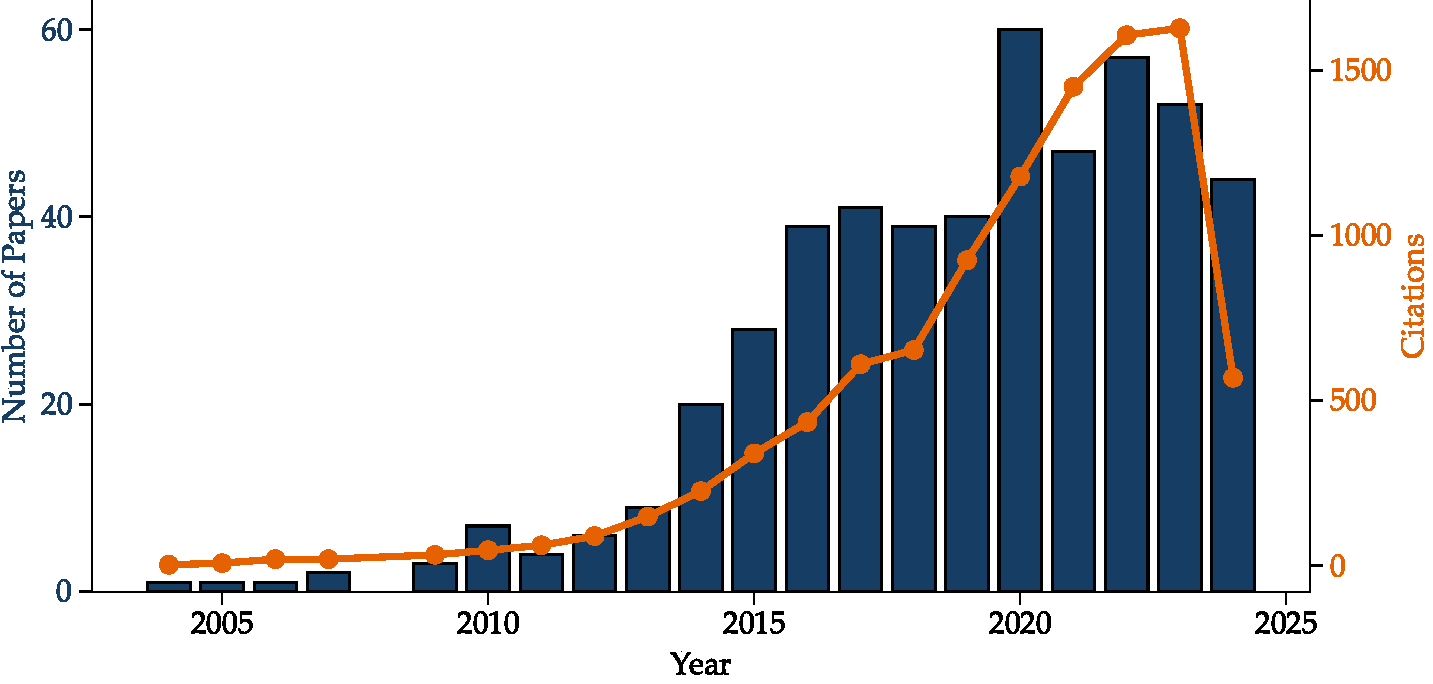
\includegraphics[width=\linewidth]{top10.pdf}
	    \caption{Published papers on hyper-reduction over the last two decades (as of 2024, \textit{source: web of science})}
\label{fig:papers}
\end{figure}

\begin{figure}[t]
	    \centering
	    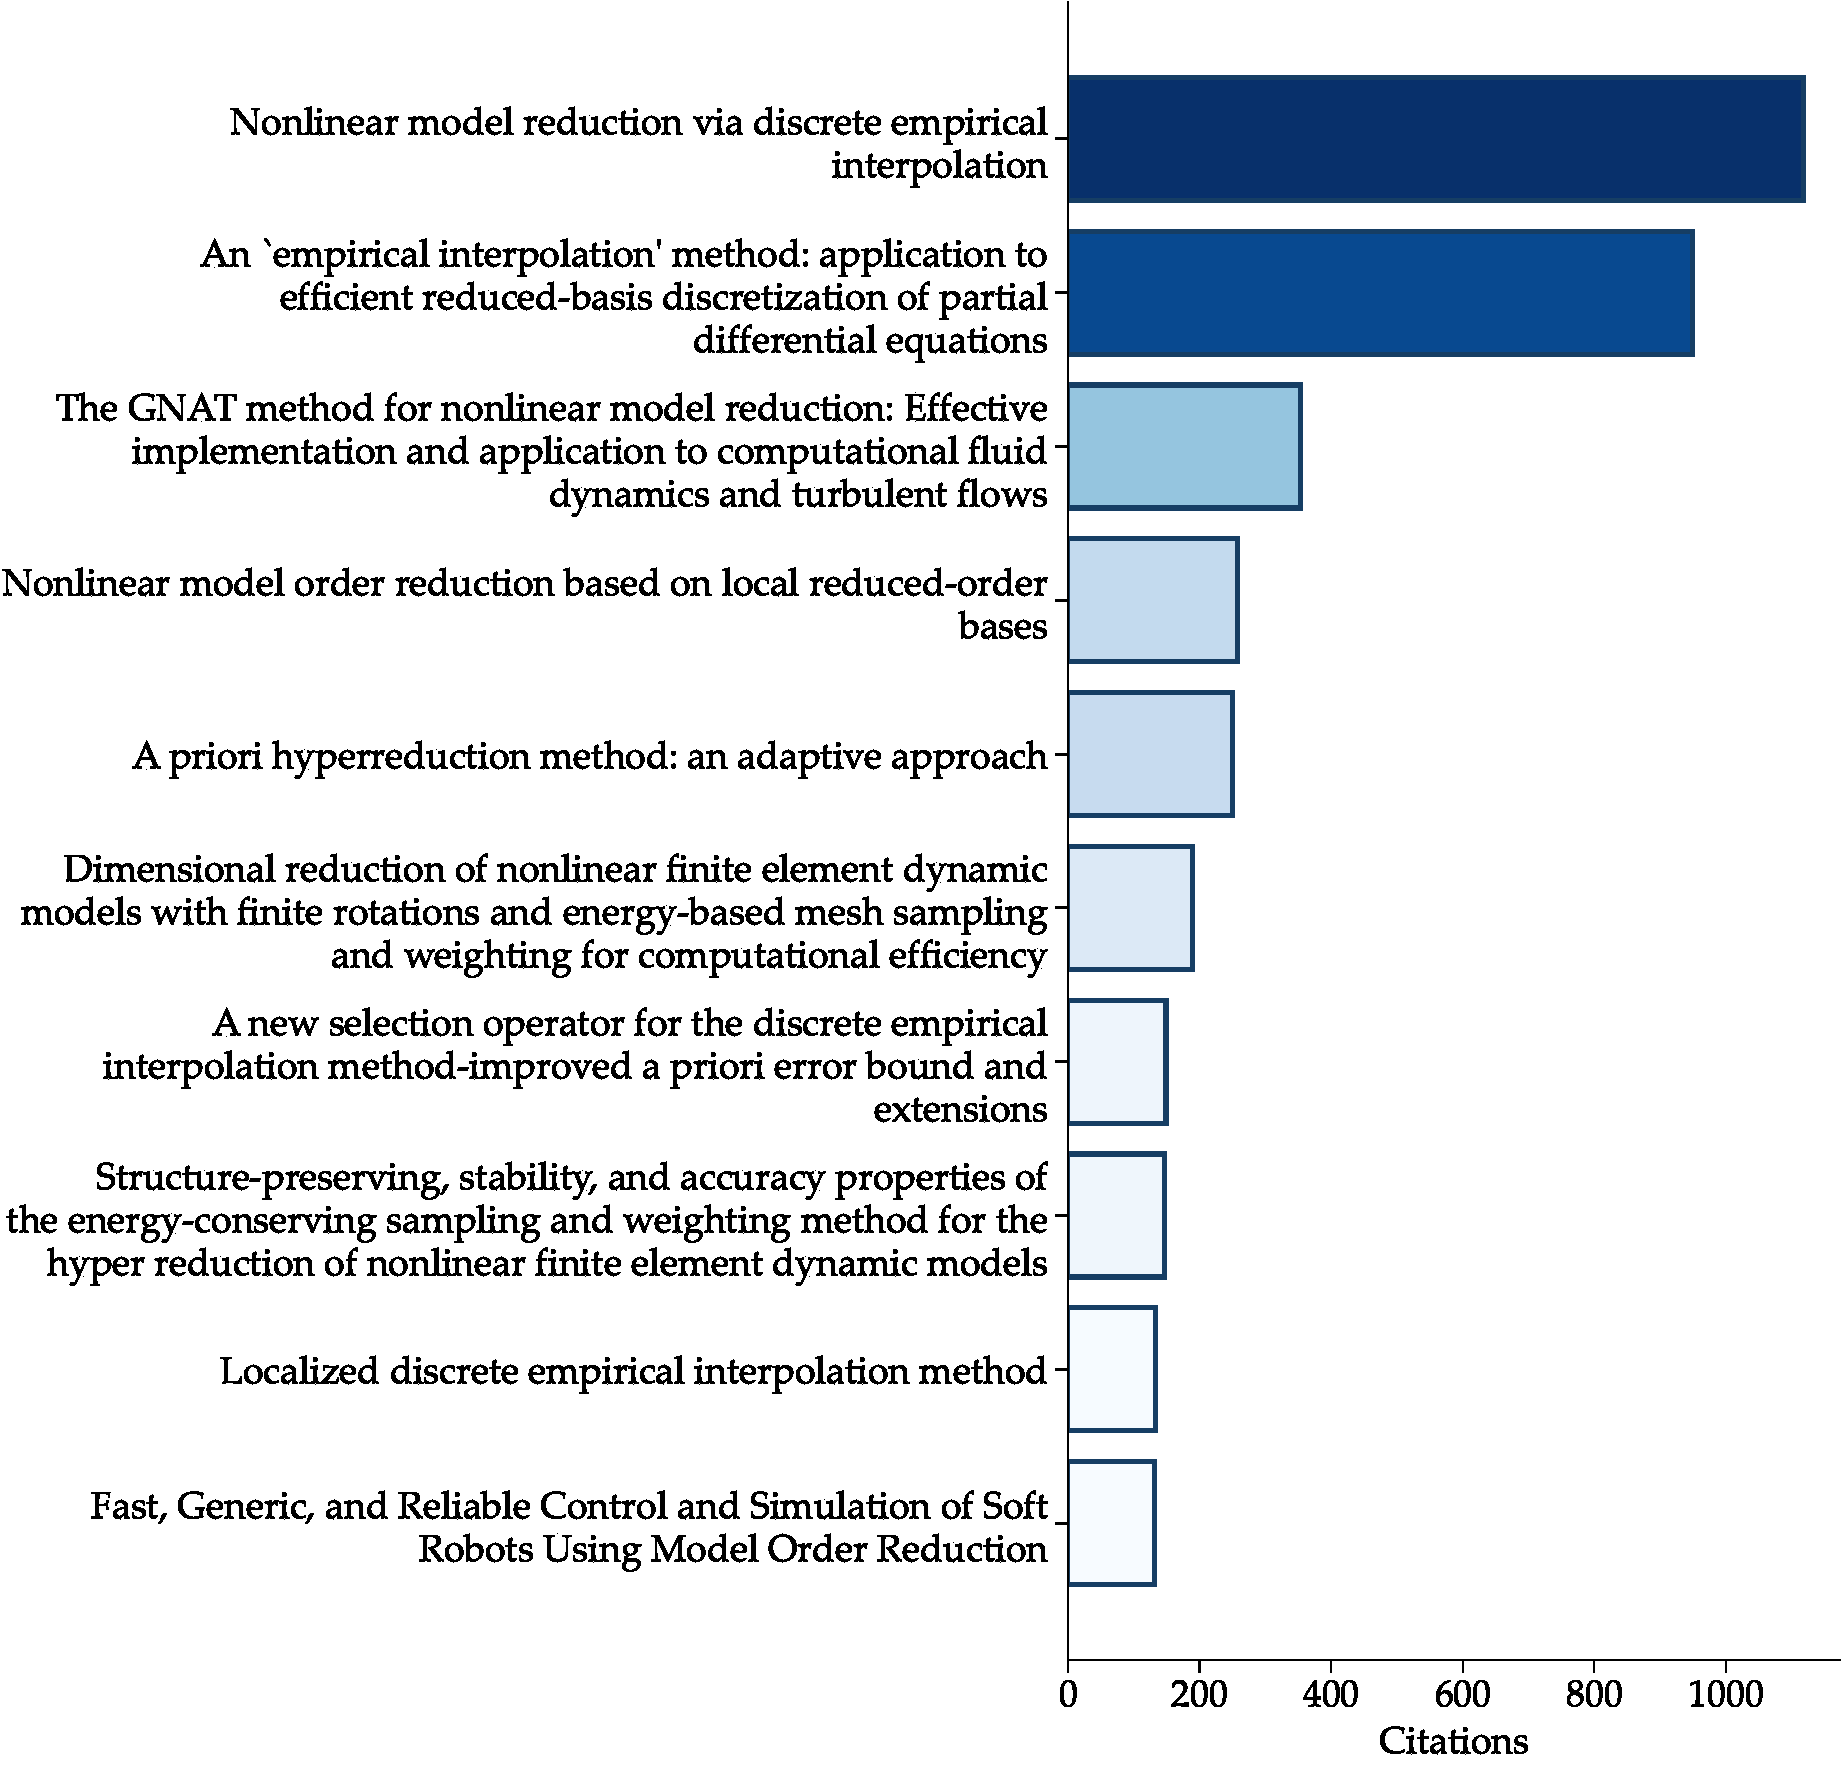
\includegraphics[width=0.8\linewidth]{papers.pdf}
	    \caption{Top 10 highly cited papers on hyper-reduction (as of 2024, \textit{source: web of science}) \cite{chaturantabut2010nonlinear,barrault2004empirical,carlberg2013gnat,amsallem2012nonlinear,ryckelynck2005priori,farhat2014dimensional,drmac2016new,farhat2015structure-preserving,peherstorfer2014localized,goury2018fast}}
\label{fig:citations}
\end{figure}

\begin{figure}[t]
    \centering
    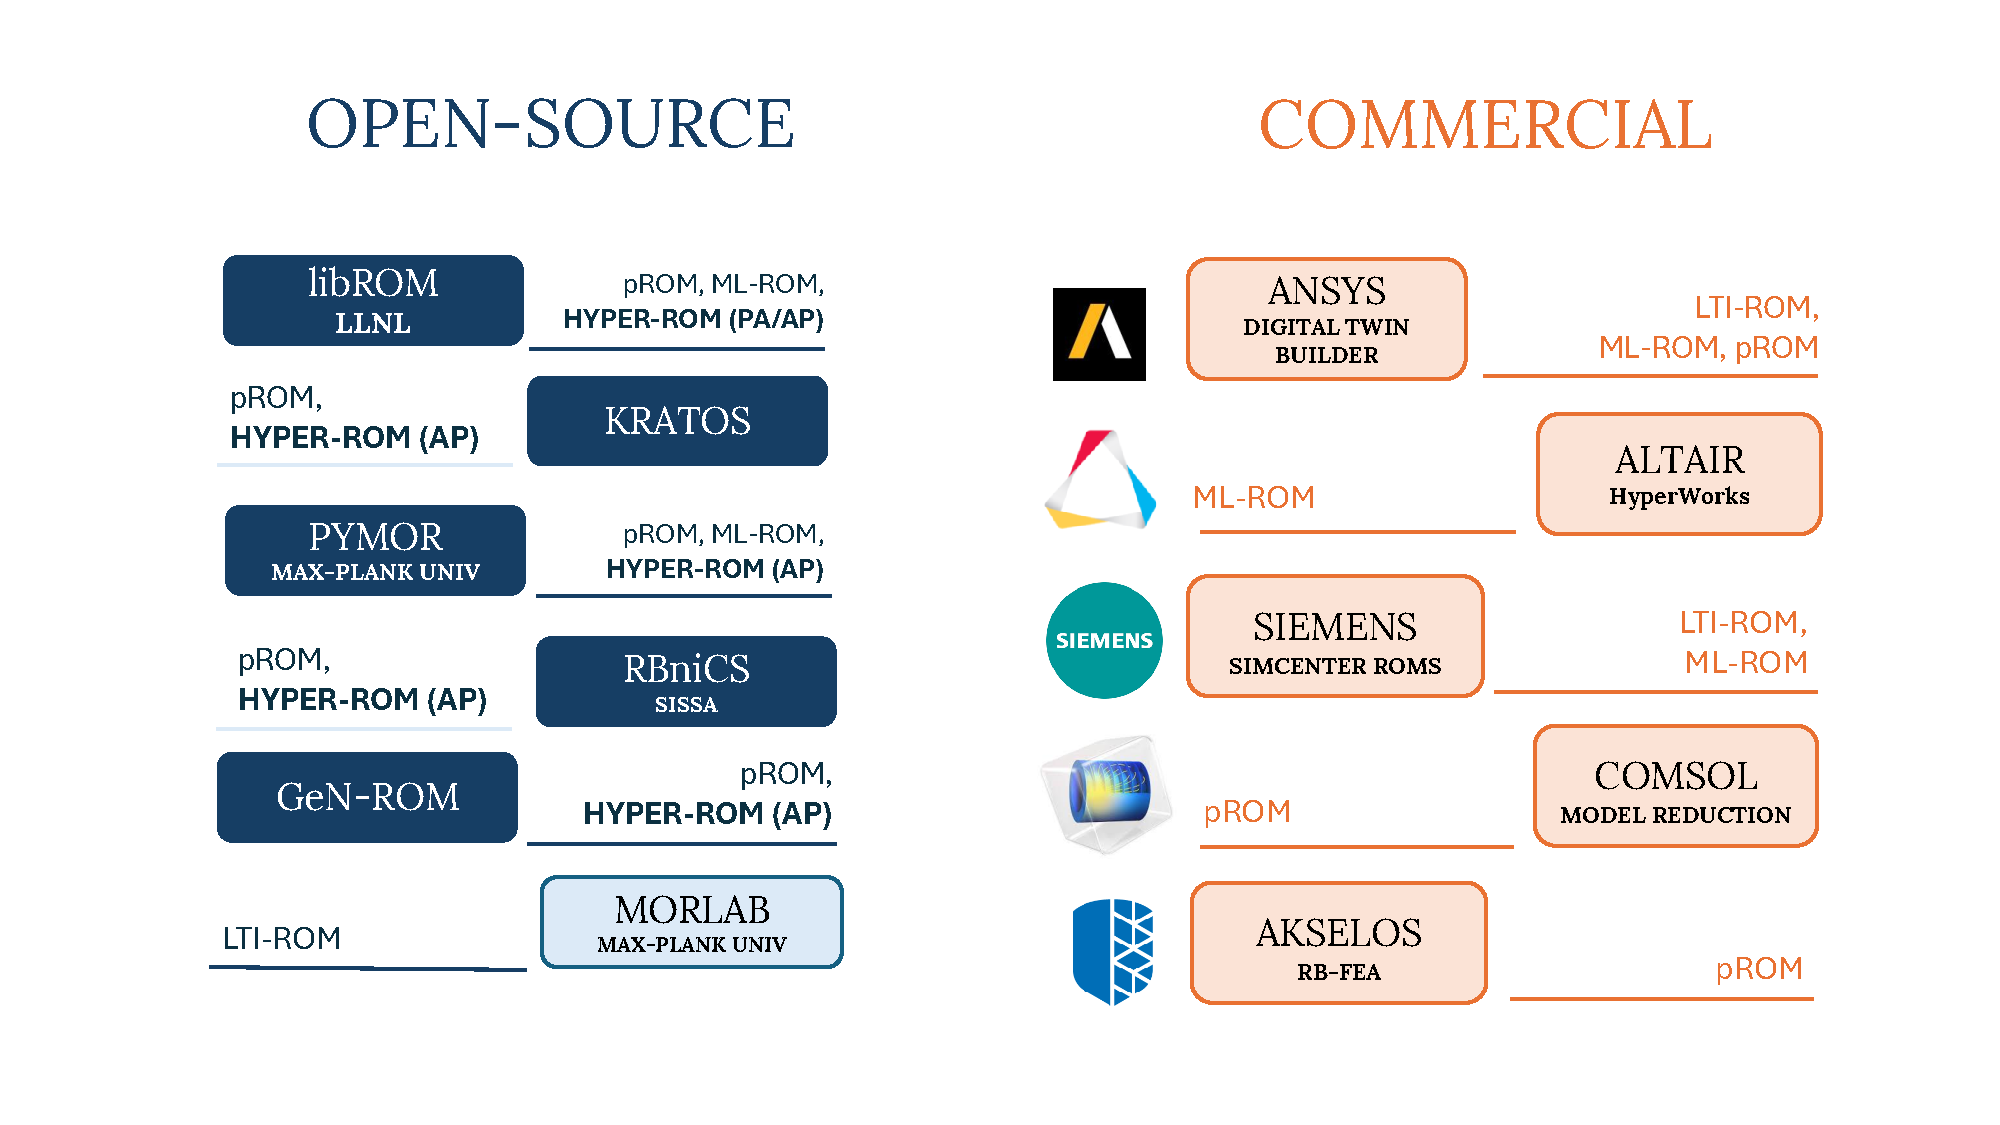
\includegraphics[width=0.9\textwidth]{software_survey5.pdf}
    \caption{Comparison of open-source and commercial software tools for reduced-order modeling (ROM) \protect\footnotemark. Open-source tools include libROM \cite{Choi2019libROM}, Kratos \cite{vicente_mataix_ferrandiz_2022_6395887}, PyMOR \cite{milk2016pymor}, RBniCS \cite{RozzaBallarinScandurraPichi2024}, and MORLAB \cite{BenW21c}. These tools support ROM methods like projection-based Reduced Order Model (pROM), Machine Learning-based ROM (ML-ROM) \cite{Drakoulas_2023,TANNOUS_2024}, Hyper-ROM (AP/PA), and Linear Time-Invariant ROM (LTI-ROM) \cite{Sikander_2017}. Dark blue boxes indicate support for Hyper-ROM, where (AP) denotes ``Approximate-then-Project,'' and (PA) denotes ``Project-then-Approximate.'' Commercial tools include ANSYS Digital Twin Builder, Altair HyperWorks, Siemens Simcenter ROMS, COMSOL Model Reduction \cite{saha2019reduced,deng2021reduced-order,Zhang_2021}, and Akselos RB-FEA \cite{Di_Nicola_2024,Sharma_2018,BRENNER_2023}, which support various ROM methods. However, none of these commercial tools support hyper-reduction.}
    \label{fig:ROM_software}
\end{figure}

\begin{figure}[t]
\centering
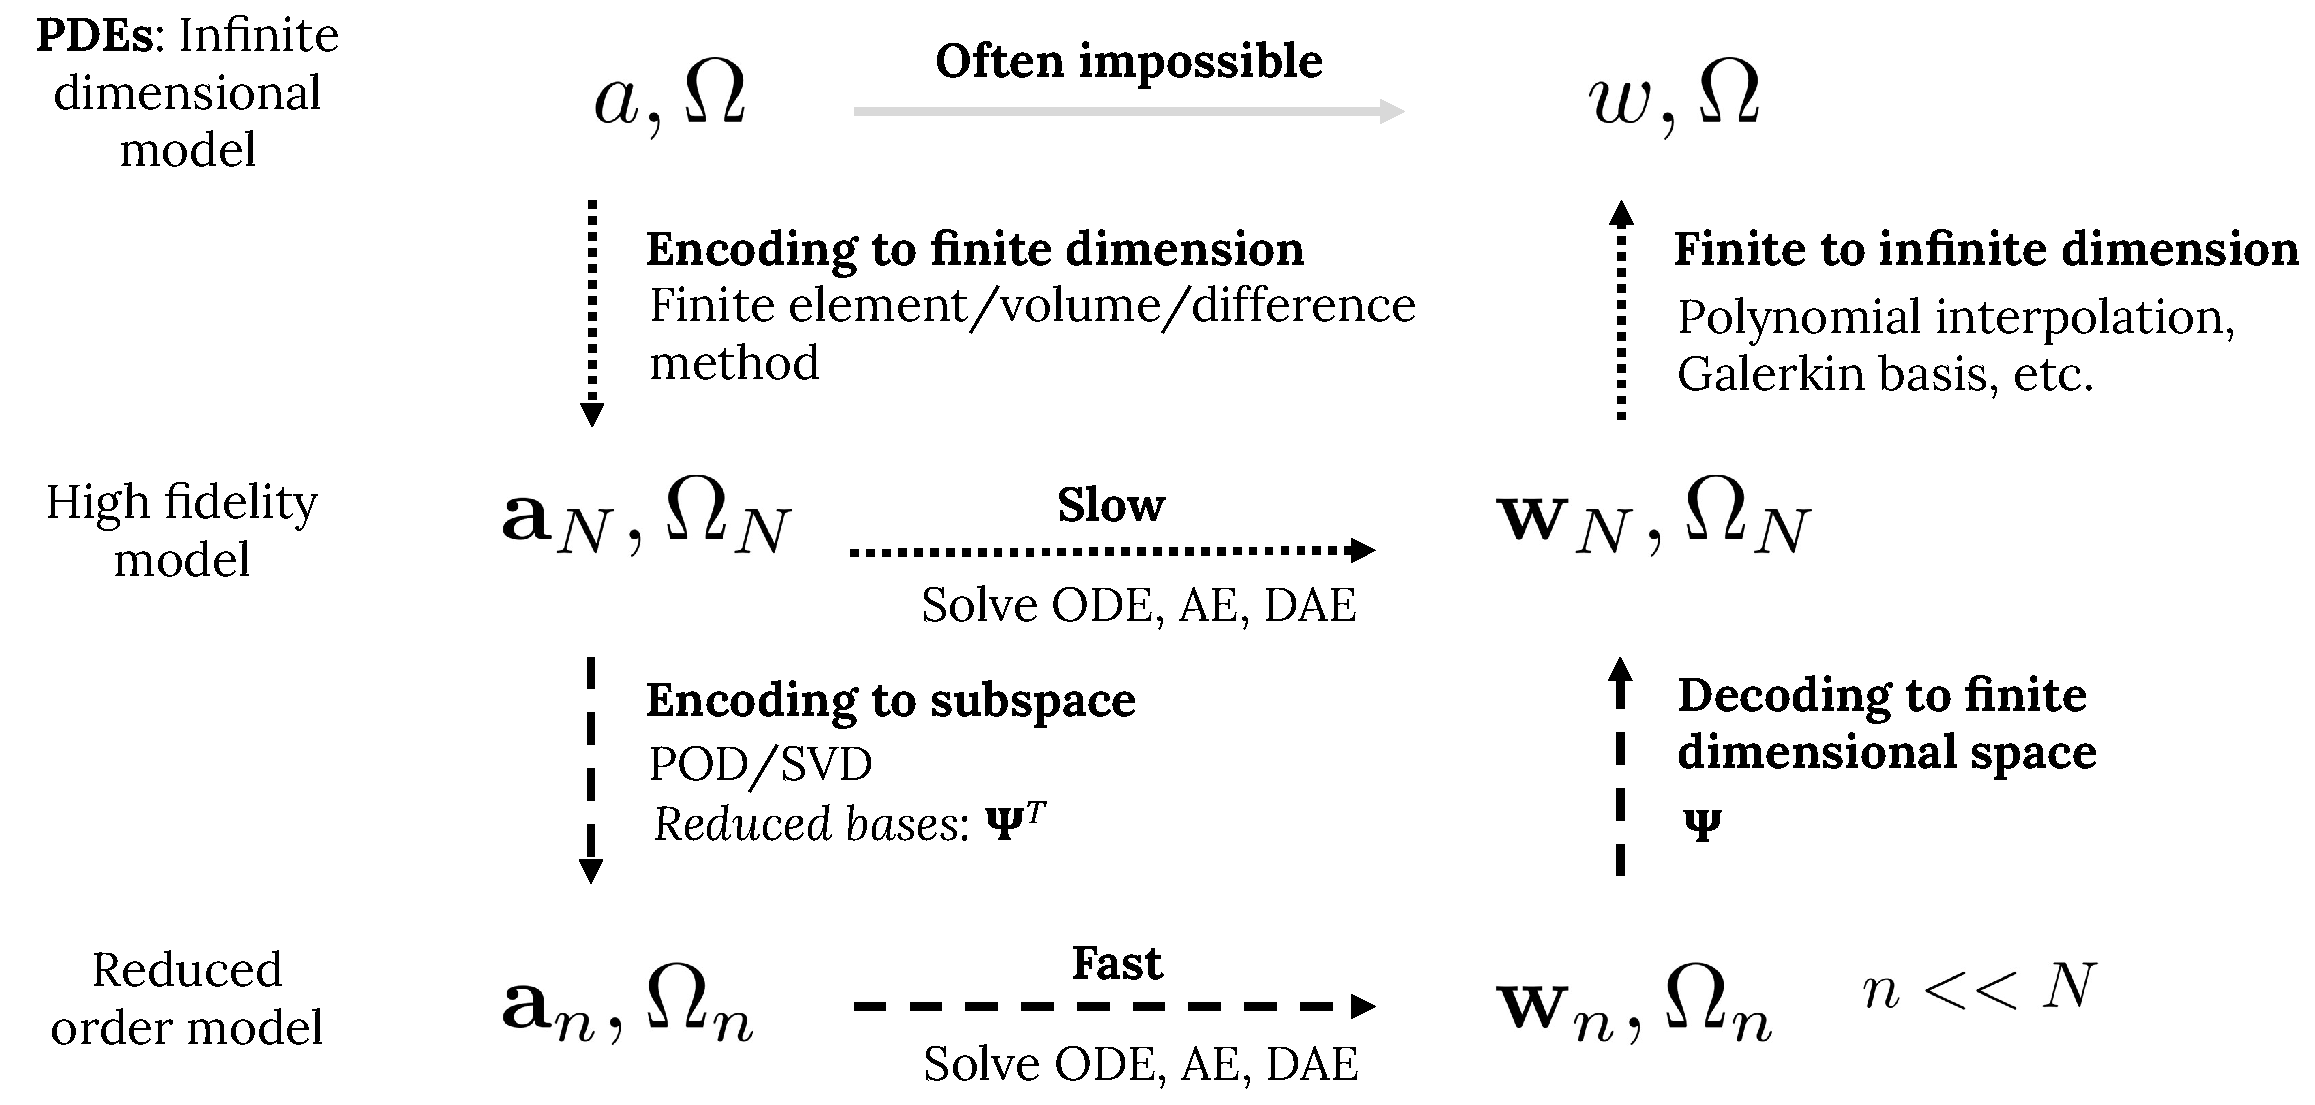
\includegraphics[width=0.8\textwidth]{schematic.pdf}
\caption{Numerical solution of PDEs. High-fidelity models and reduced order models. Here $a$ represents an input to the system; $\Omega$ is the problem domain in the infinite dimensional space, $w$ is the infinite-dimensional solution to the PDE; $\vec{a}_N$, $\vec{w}_N$ and $\Omega_N$ are the high-dimensional finite approximation, and $\vec{a}_n$, $\vec{w}_n$ and $\Omega_n$ are the reduced representation of  $\vec{a}$, $\Omega$, and $\vec{w}$, respectively.}
\label{fig:ROM_FOM_schematic}
\end{figure}

\begin{figure}[t]
    \centering
    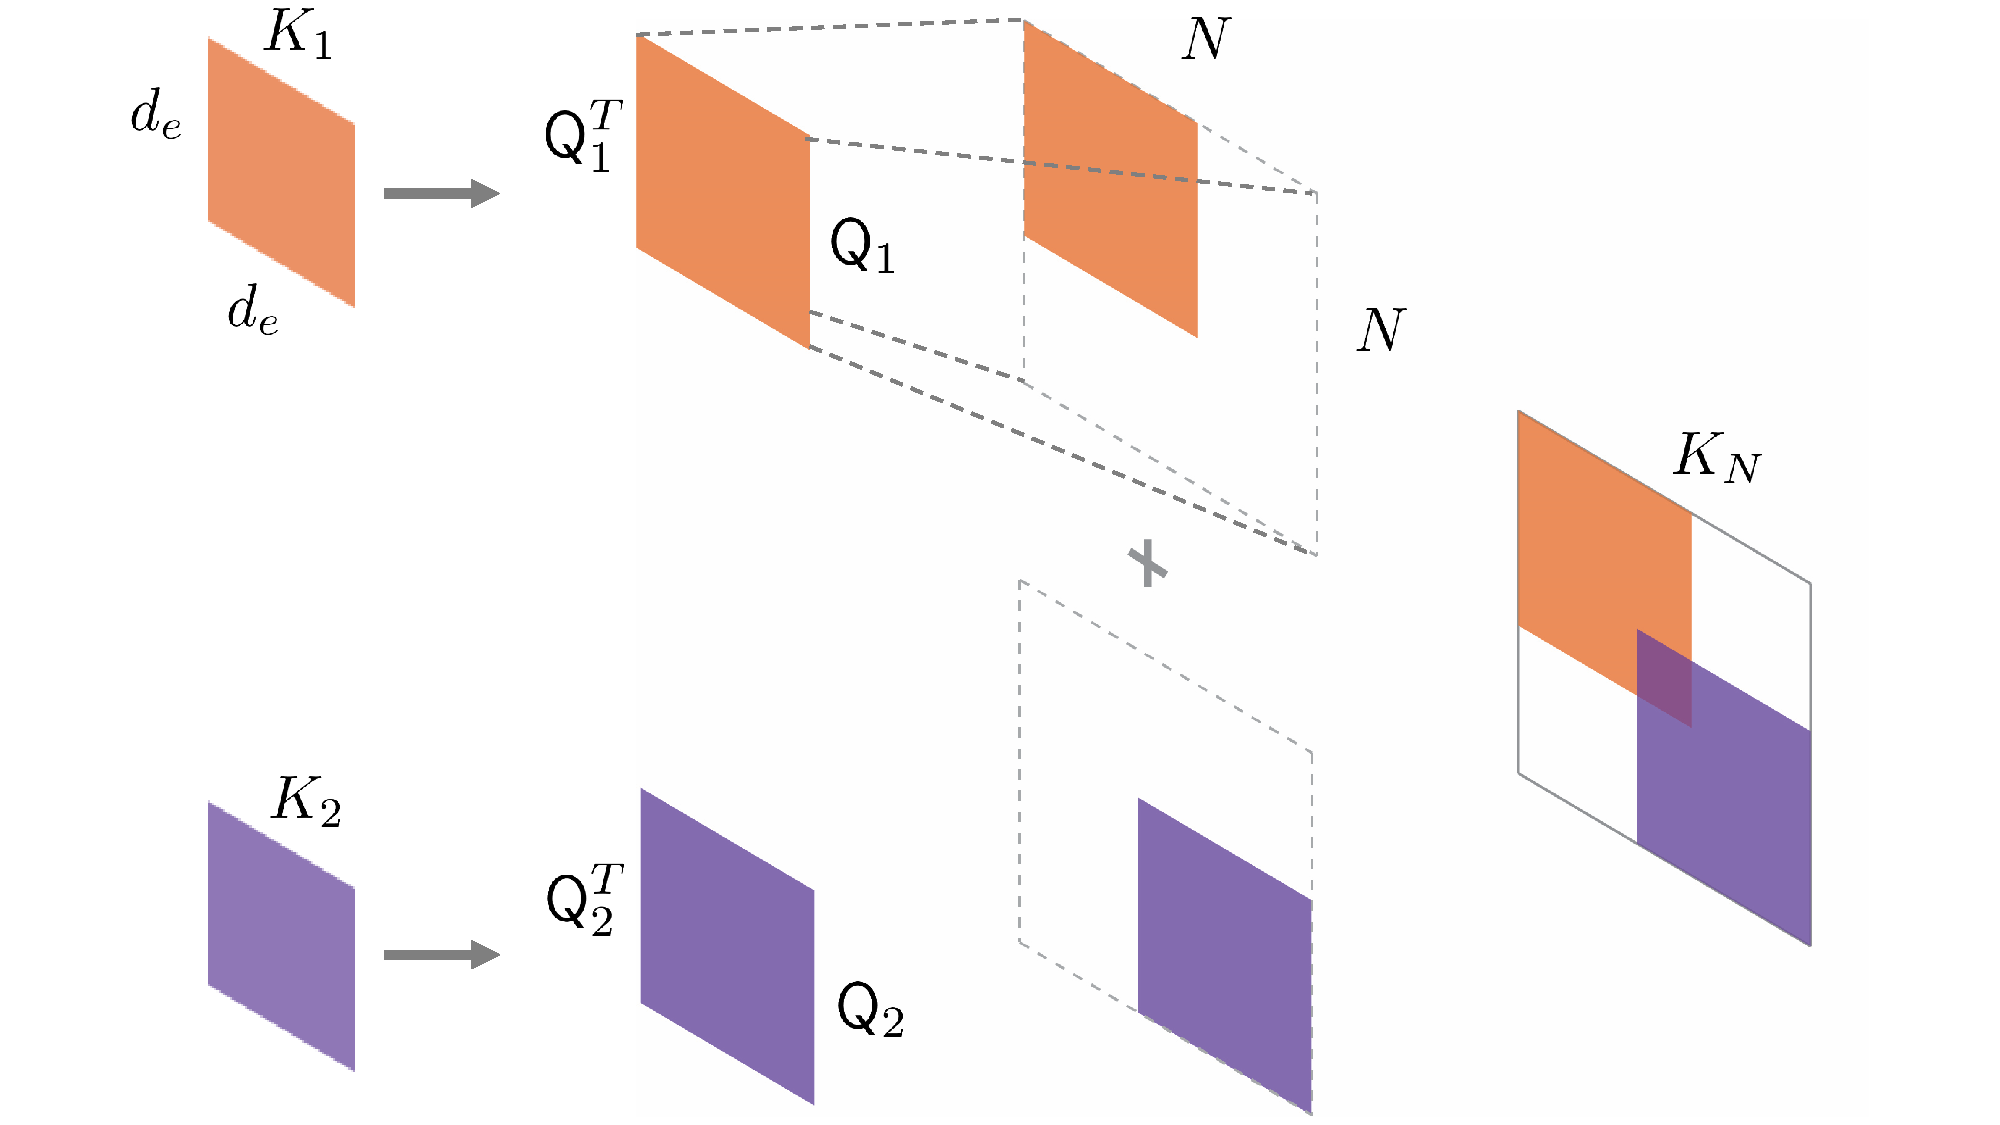
\includegraphics[width=0.6\linewidth]{K_full.pdf}
    \caption{Visual representation of the assembly of elemental stiffness matrices for the finite element model of the toy problem in Sec.~3. Local stiffness matrices \( \mat{K}_1 \) and \( \mat{K}_2 \), corresponding to individual finite elements, are transformed into the global coordinate system using their respective transformation matrices \( \mat{Q}_1 \) and \( \mat{Q}_2 \). These transformations expand the local matrices into the global framework, mapping local degrees of freedom to the global degrees of freedom. The global stiffness matrix \( \mat{K}_N \) is then constructed by adding these transformed matrices, summing contributions from overlapping degrees of freedom. Color-coded blocks highlight each local matrix's contribution to the global system.}
    \label{fig:visual_FOM_FEA}
\end{figure}

\begin{figure}[t]
\centering
\begin{subfigure}[b]{0.45\linewidth}
\centering
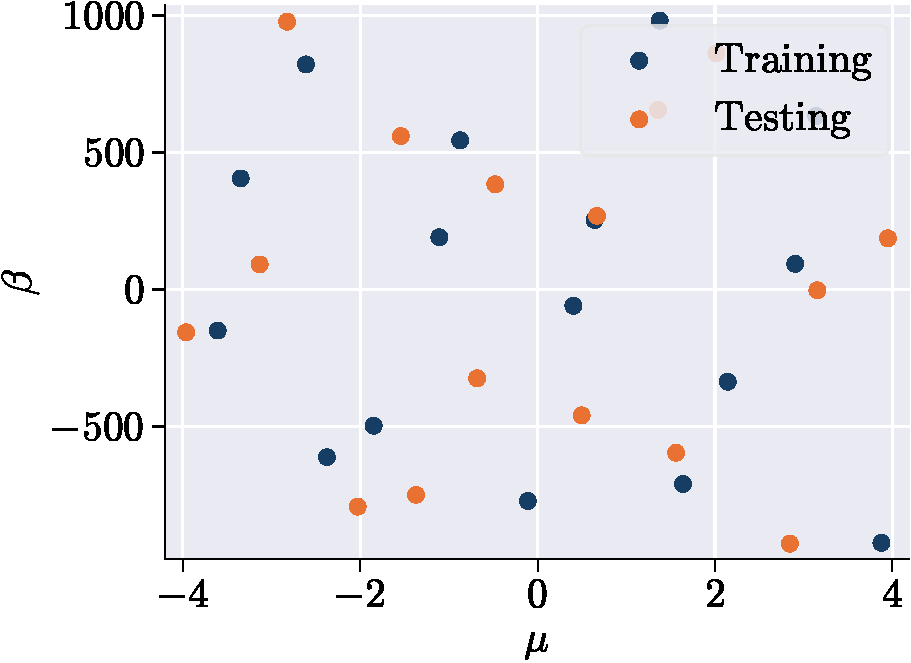
\includegraphics[width=\linewidth]{param_list_L.pdf}
\caption{}
\label{fig:HFS_HC_a}
\end{subfigure}
\begin{subfigure}[b]{0.45\linewidth}
\centering
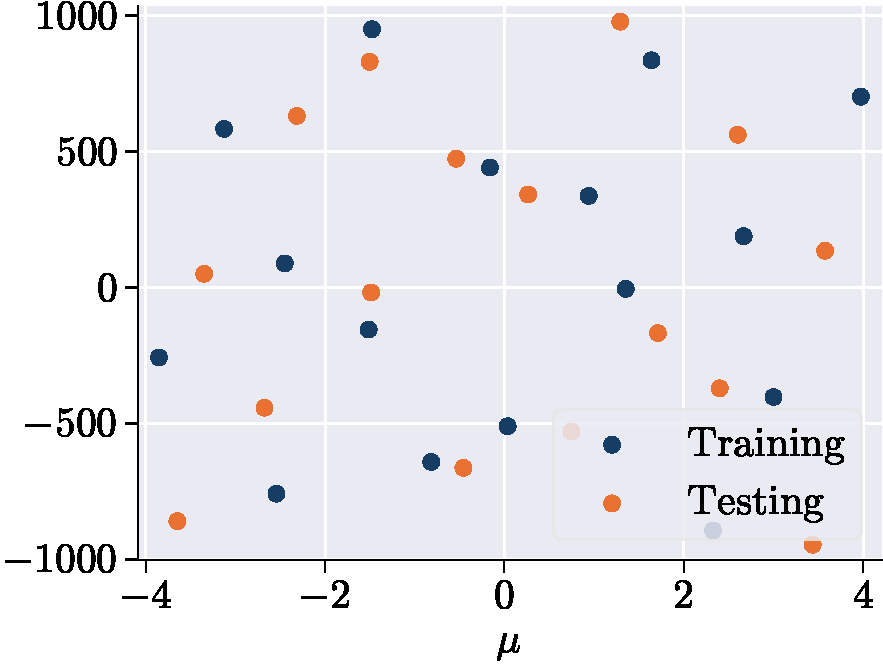
\includegraphics[width=0.98\linewidth]{param_list_NL.pdf}
\caption{}
\label{fig:HFS_HC_b}
\end{subfigure}

\begin{subfigure}[b]{0.45\linewidth}
\centering
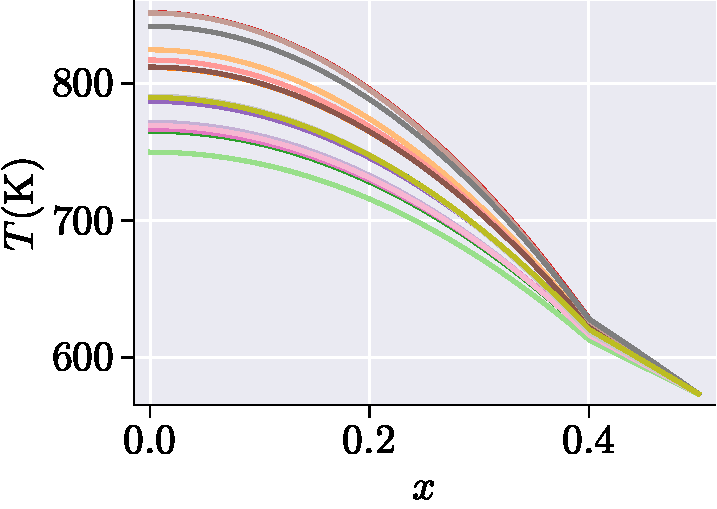
\includegraphics[width=\linewidth]{linear_T_FOM.pdf}
\caption{}
\label{fig:HFS_HC_c}
\end{subfigure}
\begin{subfigure}[b]{0.45\linewidth}
\centering
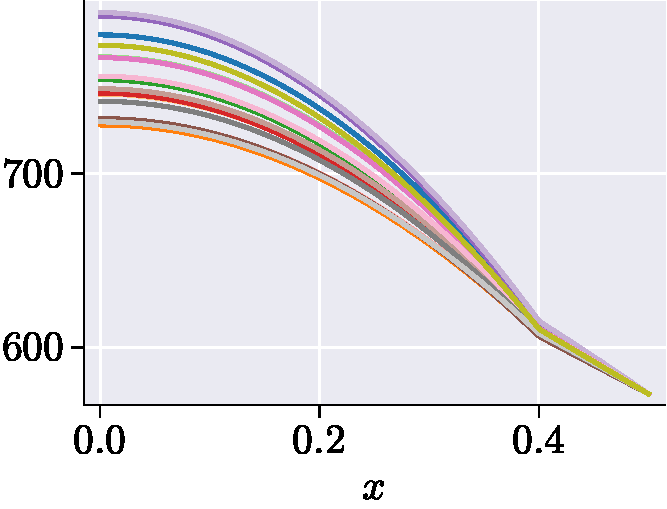
\includegraphics[width=0.92\linewidth]{nonlinear_T_FOM.pdf}
\caption{}
\label{fig:HFS_HC_d}
\end{subfigure}
\caption{High Fidelity solution snapshots for the linear and the nonlinear system corresponding to different values of the thermal conductivity and heat source values as defined in \cref{eq:k_mu_L,eq:k_mu_NL,eq:q_beta}.
Variation in the parameters for the linear system is shown in (a) and (c), and for the nonlinear system is shown in (b) and (d).
Here the parameter pairs are selected based on the sobol sequence, which explores the entire parameter space.}
\label{fig:HFS_HC}
\end{figure}

\begin{figure}[t]
\centering
\begin{subfigure}[b]{0.45\linewidth}
\centering
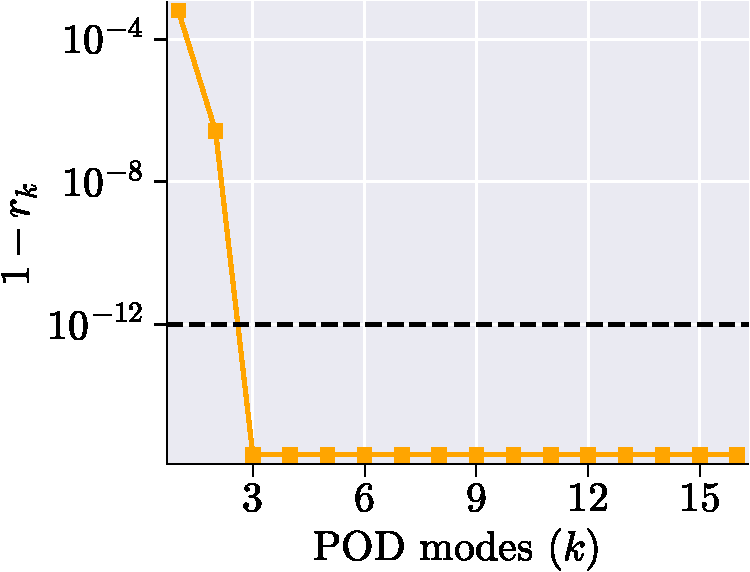
\includegraphics[width=\linewidth]{linear_Mode_selection.pdf}
\caption{}
\label{fig:HC_ROM_a}
\end{subfigure}
\begin{subfigure}[b]{0.45\linewidth}
\centering
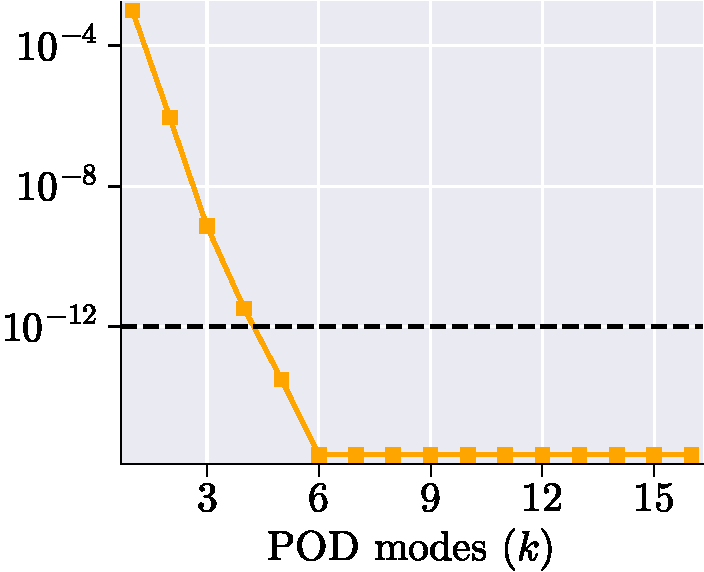
\includegraphics[width=0.93\linewidth]{nonlinear_Mode_selection.pdf}
\caption{}
\label{fig:HC_ROM_b}
\end{subfigure}

\begin{subfigure}[b]{0.45\linewidth}
\centering
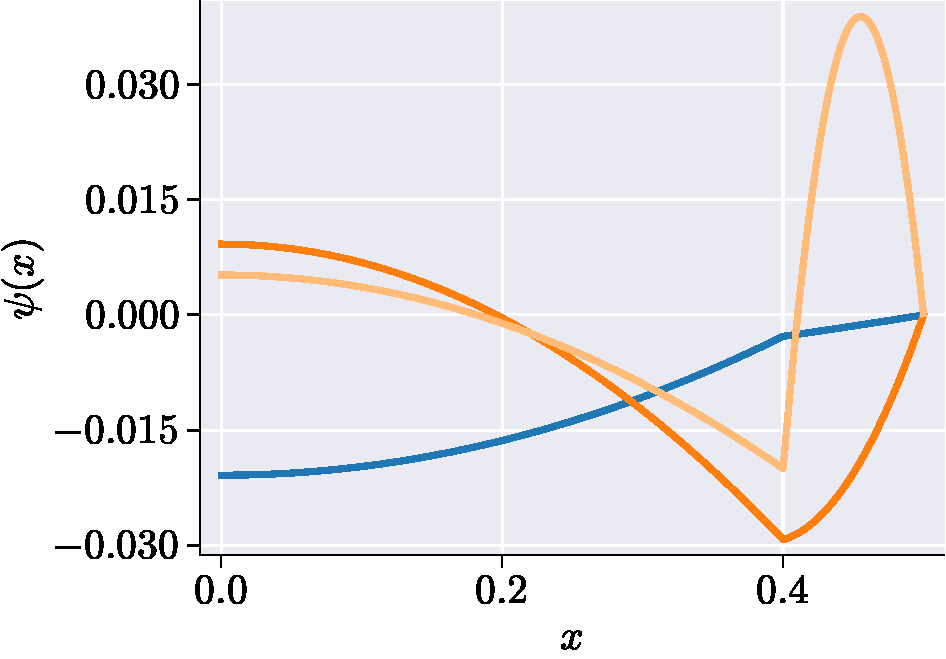
\includegraphics[width=\linewidth]{linear_Mode_shapes.pdf}
\caption{}
\label{fig:HC_ROM_c}
\end
{subfigure}
\begin{subfigure}[b]{0.45\linewidth}
\centering
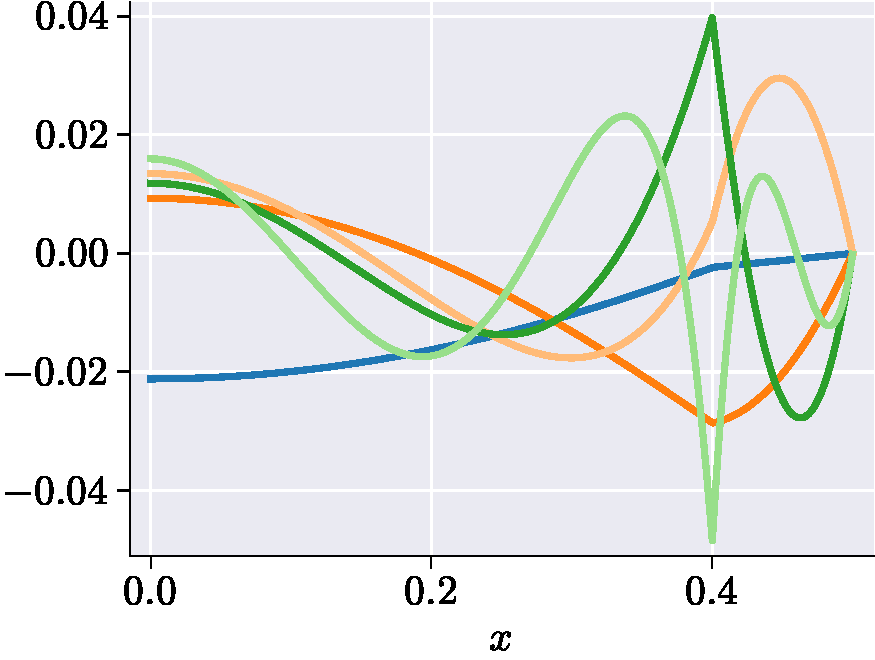
\includegraphics[width=0.96\linewidth]{nonlinear_Mode_shapes.pdf}
\caption{}
\label{fig:HC_ROM_d}
\end{subfigure}
\caption{Singular values and left reduced-order basis (ROB) obtained from the solution snapshots of  the linear (left column) and nonlinear (right column) problems.
Figures (a) and (b) display the decay of the singular values, with the dashed line indicating the chosen tolerance threshold, while (c) and (d) depict the corresponding spatial modes of the left ROB.}
\label{fig:HC_ROM}
\end{figure}

\begin{figure}[t]
\centering
\begin{subfigure}[b]{0.47\linewidth}
\centering
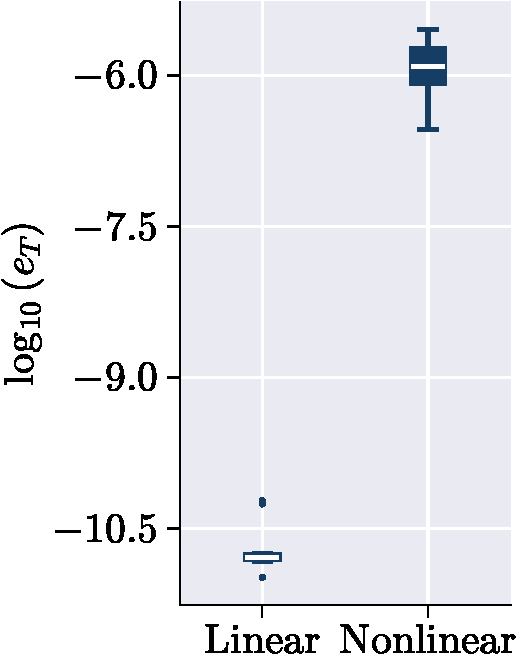
\includegraphics[height=0.95\linewidth]{error_comp.pdf}
\caption{}
\label{fig:HC_ERROR_SPDUP_c}
\end{subfigure}\hfill
\begin{subfigure}[b]{0.47\linewidth}
\centering
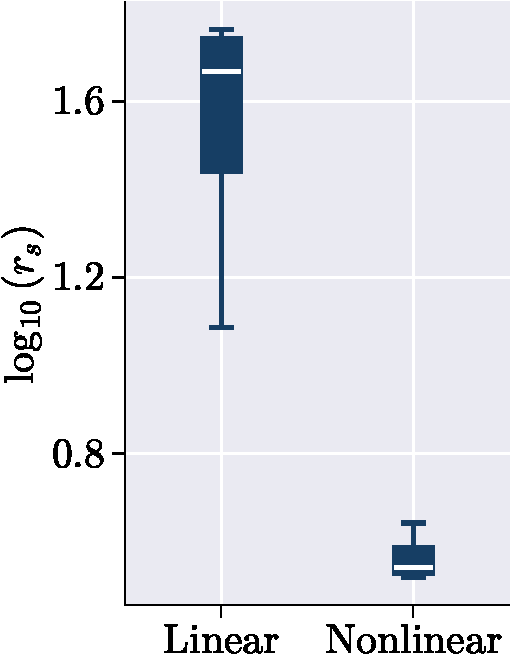
\includegraphics[height=0.95\linewidth]{speed_up_comp.pdf}
\caption{}
\label{fig:HC_ERROR_SPDUP_d}
\end{subfigure}
\caption{Difference in accuracy ($e_T$) and speed-up ($r_s$) between projection based linear and nonlinear ROMs.}
\label{fig:HC_ERROR_SPDUP}
\end{figure}

\begin{figure}
\centering
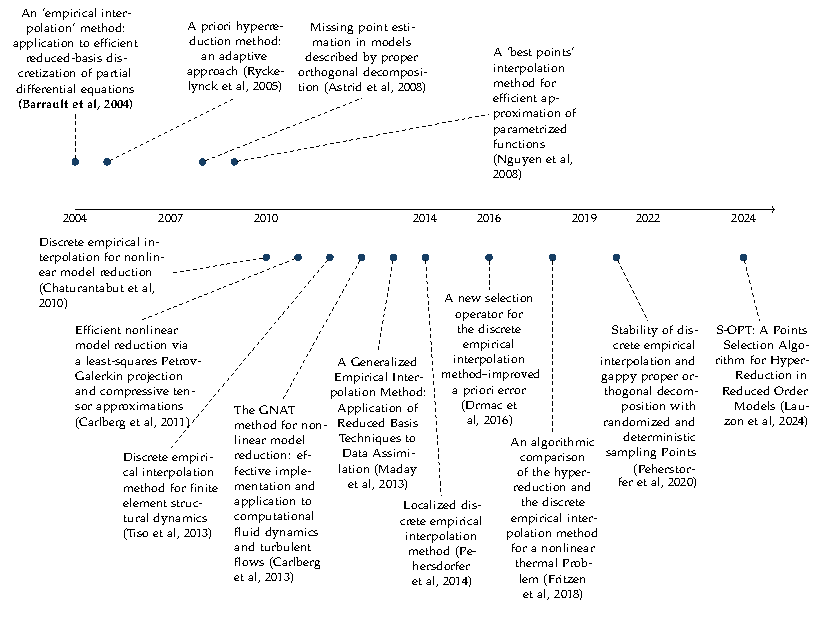
\includegraphics[width=\textwidth]{ATP.pdf}
\caption{Timeline of Seminal Papers on Approximate-then-Project hyper-reduction Algorithms. \cite{barrault2004empirical,ryckelynck2005priori,nguyen2007best,astrid2008missing,chaturantabut2010nonlinear,carlberg2011efficient,tiso2013discrete,carlberg2013gnat,peherstorfer2014localized,drmac2016new,peherstorfer2020stability,lauzon2024s-opt,Fritzen_2018,Maday_2013}.}
\label{fig:ATP_LIT}
\end{figure}

\begin{figure}[t]
    \centering
    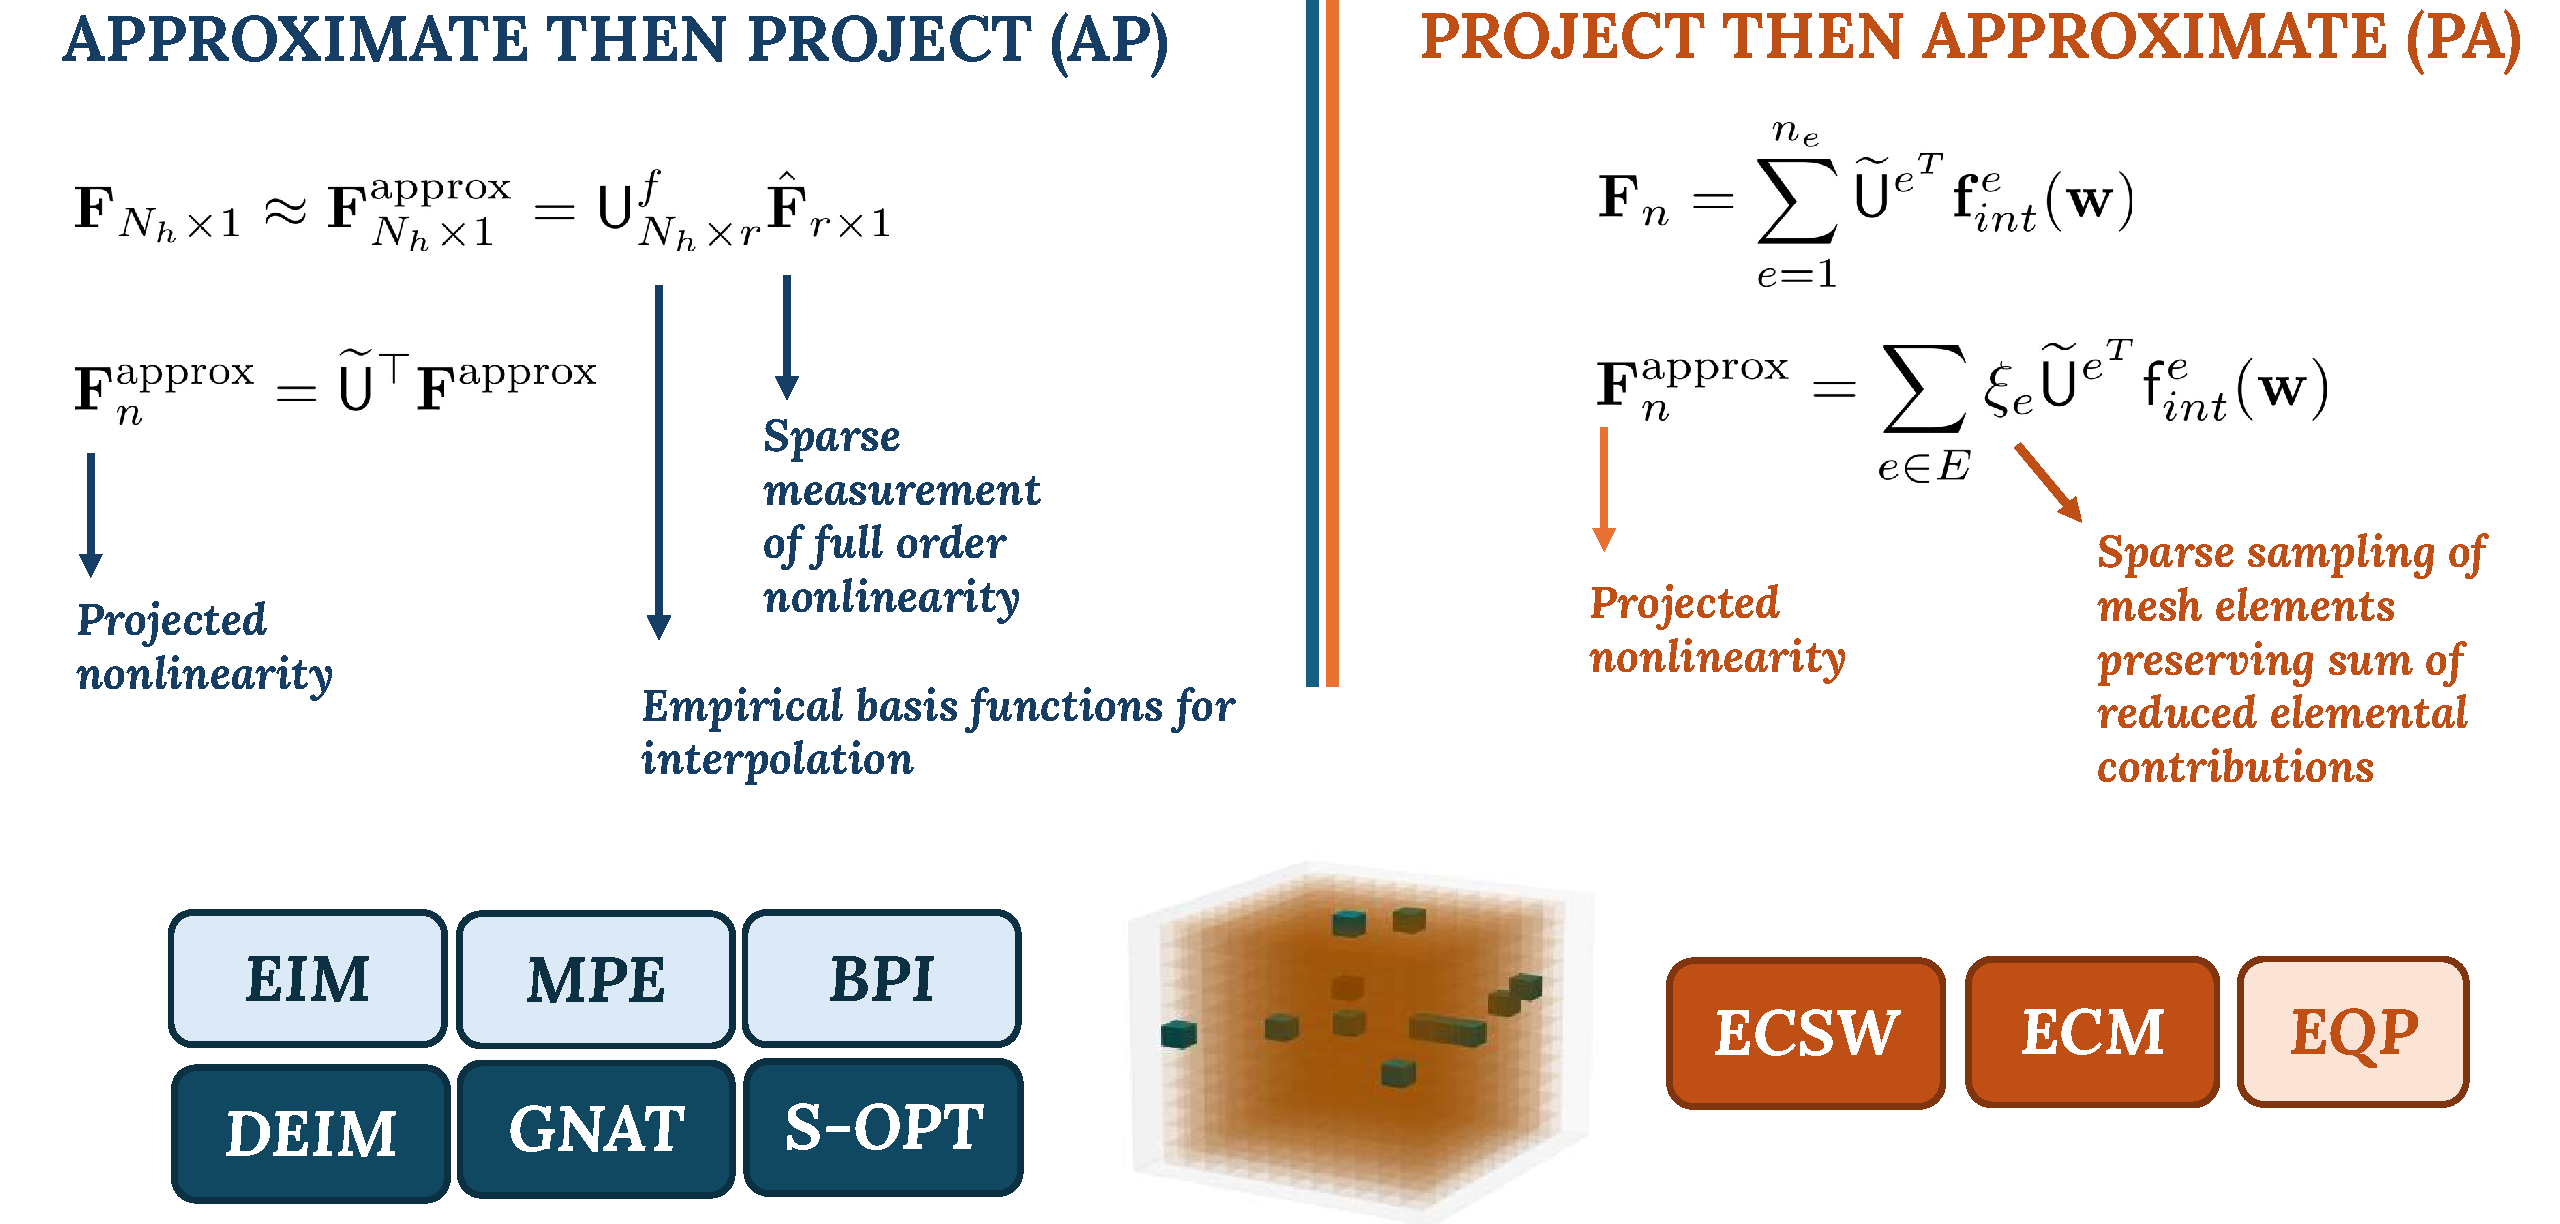
\includegraphics[width=\linewidth]{ATP_PTA2.pdf}
    \caption{Classification of hyper-reduction algorithms \protect\footnotemark(EIM: Empirical Interpolation Method \cite{barrault2004empirical}, MPE: Missing Point Estimation \cite{astrid2008missing}, BPI: Best Point Interpolation \cite{nguyen2007best}, DEIM: Discrete Empirical Interpolation Method \cite{chaturantabut2010nonlinear}, GNAT: Gauss-Newton Approximation Tensor \cite{carlberg2011efficient}, S-OPT: S-optimality based point selection \cite{lauzon2024s-opt}, ECSW: Energy Conserving Sampling and Weighing \cite{farhat2014dimensional}, ECM: Empirical Cubature Method \cite{hernandez2017dimensional}, EQP: Empirical Quadrature Procedure \cite{Patera_2017_EQP}): Approximate Then Project (AP) and Project Then Approximate (PA). In the AP approach, sparse measurements of the full-order nonlinearity are used in conjunction with empirical basis functions for interpolation, approximating the projected nonlinearity. In contrast, the PA approach involves projecting nonlinearity first and then employing sparse sampling of mesh elements to preserve the sum of reduced elemental contributions. Boxes with darker backgrounds, including DEIM, S-OPT, ECSW, and ECM are specifically discussed in the paper.}
    \label{fig:hyp_algo}
\end{figure}

\begin{figure}[t!]
    \centering
    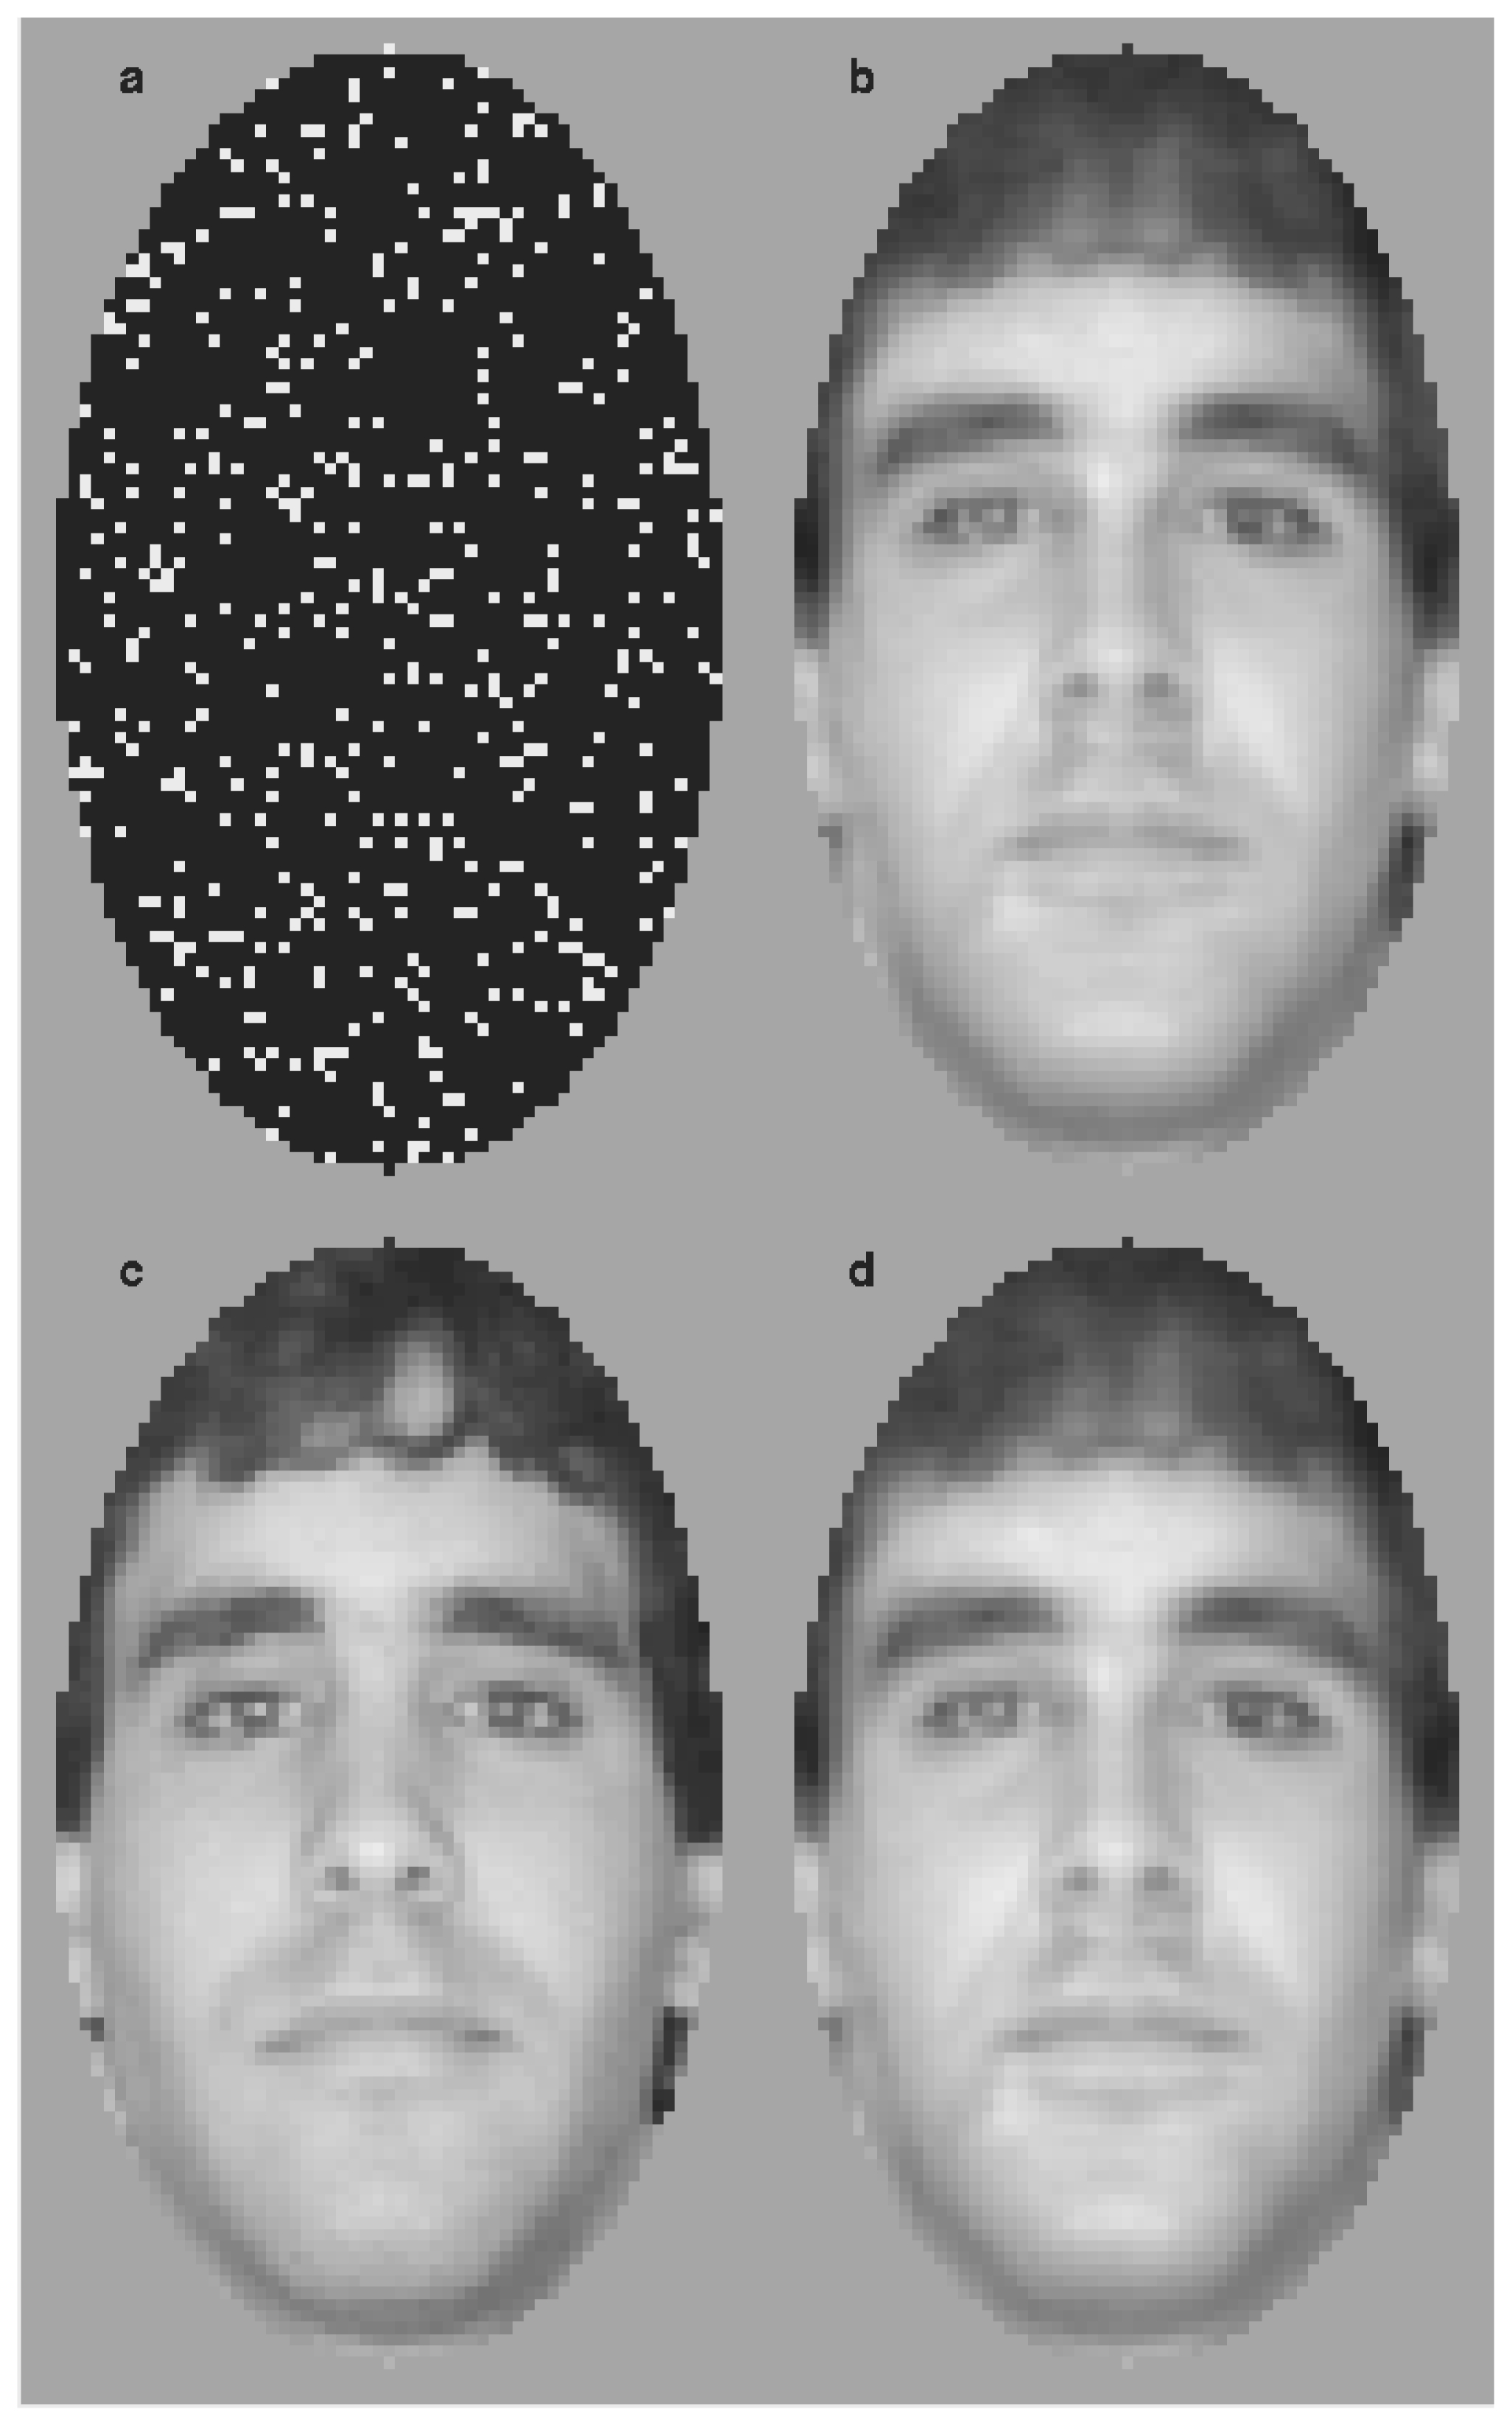
\includegraphics[width=0.25\linewidth]{gappy_pod2.jpg}
    \caption{Reconstruction of marred images using Gappy-POD \cite{sirovich1987low-dimensional}.}
\label{fig:pic_db}
\end{figure}

\begin{figure}[t]
\centering
\begin{subfigure}[b]{0.45\linewidth}
\centering
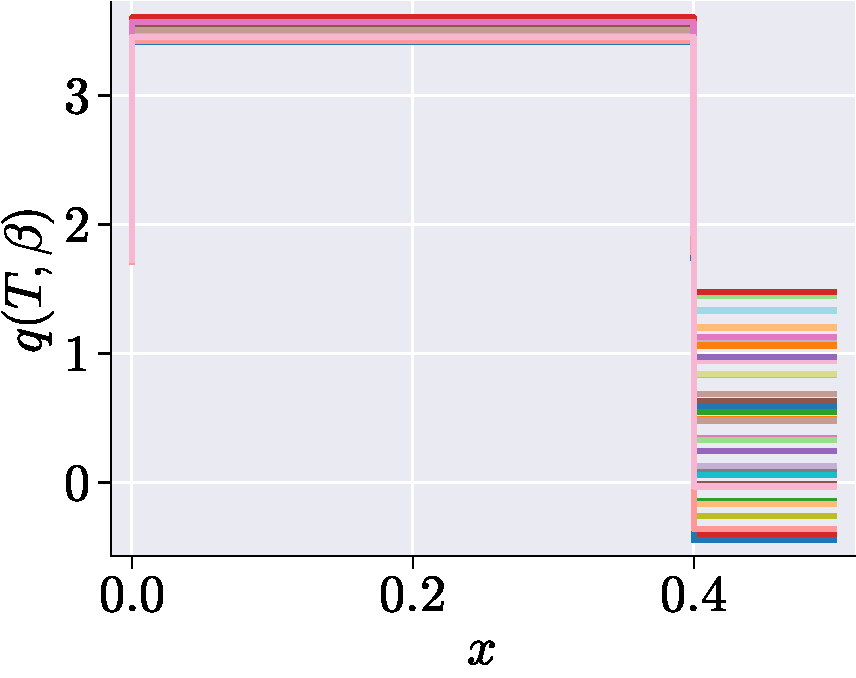
\includegraphics[width=\linewidth]{DEIM_snapshots.pdf}
\caption{}
\label{fig:DEIM_snap_a}
\end{subfigure}
\begin{subfigure}[b]{0.45\linewidth}
\centering
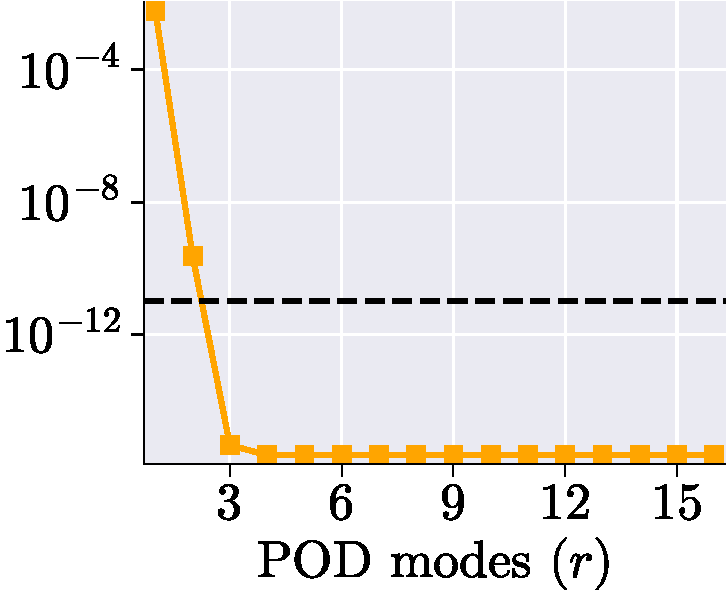
\includegraphics[width=0.97\linewidth]{DEIM_SVs.pdf}
\caption{}
\label{fig:DEIM_snap_b}
\end{subfigure}
\caption{The snapshots of the source function corresponding to various parameter values used for DEIM are shown in (a).
In (b), the decay of singular values, obtained by applying SVD on the snapshots, is illustrated.
This decay informs the selection of the number of singular vectors, \( r \), to use in the DEIM algorithm.
Here, \( r = 4 \) was selected.}
\label{fig:DEIM_snap}
\end{figure}

\begin{figure}[t]
    \centering
    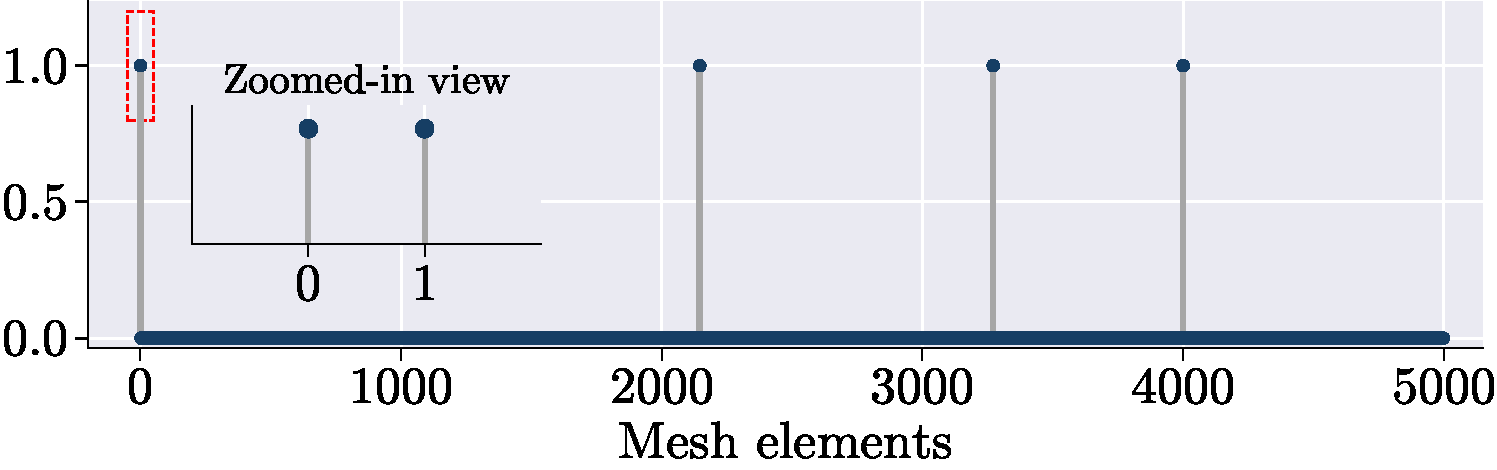
\includegraphics[width=0.8\linewidth]{reduced_mesh_DEIM_new.pdf}
    \caption{The reduced mesh obtained using DEIM. Excluded  elements lie on the blue line. As shown in the inset, for each DEIM point, all associated elements (in this case, two per point) are selected. The resulting reduced mesh in this case comprises only 8 elements, which constitutes 0.16\% of the total 5,000 elements in the original high-fidelity model.}
    \label{fig:reduced_mesh_deim}
\end{figure}

\begin{figure}[t!]
\centering
\begin{subfigure}[b]{0.47\linewidth}
\centering
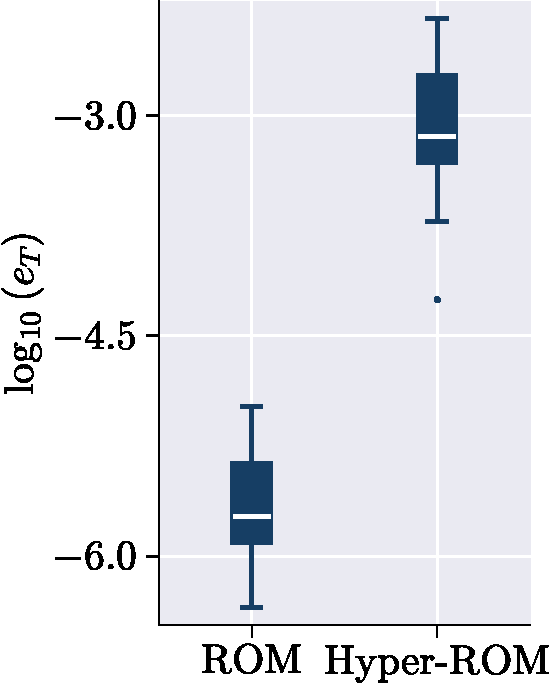
\includegraphics[height=0.95\linewidth]{error_comp_rom_hrom_deim.pdf}
\caption{}
\label{fig:HROM_ERROR_SPDUP_a_deim}
\end{subfigure}\hfill
\begin{subfigure}[b]{0.47\linewidth}
\centering
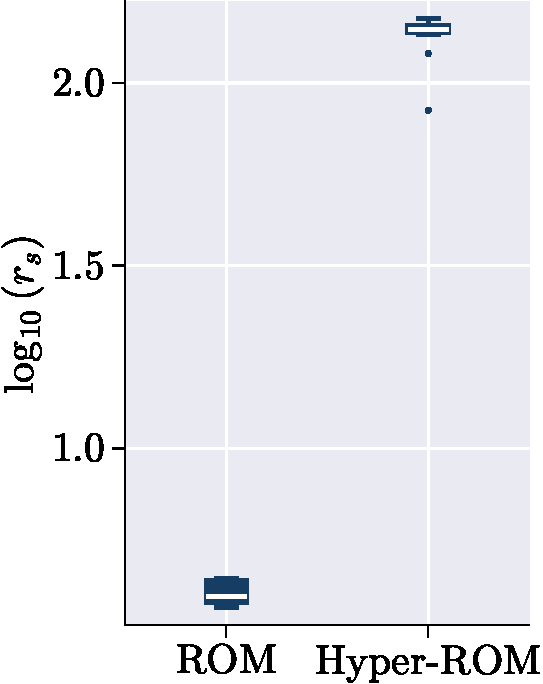
\includegraphics[height=0.95\linewidth]{speed_up_comp_rom_hrom_deim.pdf}
\caption{}
\label{fig:HROM_ERROR_SPDUP_b_deim}
\end{subfigure}
\caption{Difference in accuracy ($e_T$) and speed-up ($r_s$) between the regular projection based ROM and Hyper-ROM.}
\label{fig:HROM_ERROR_SPDUP_deim}
\end{figure}

\begin{figure}[t]
    \centering
    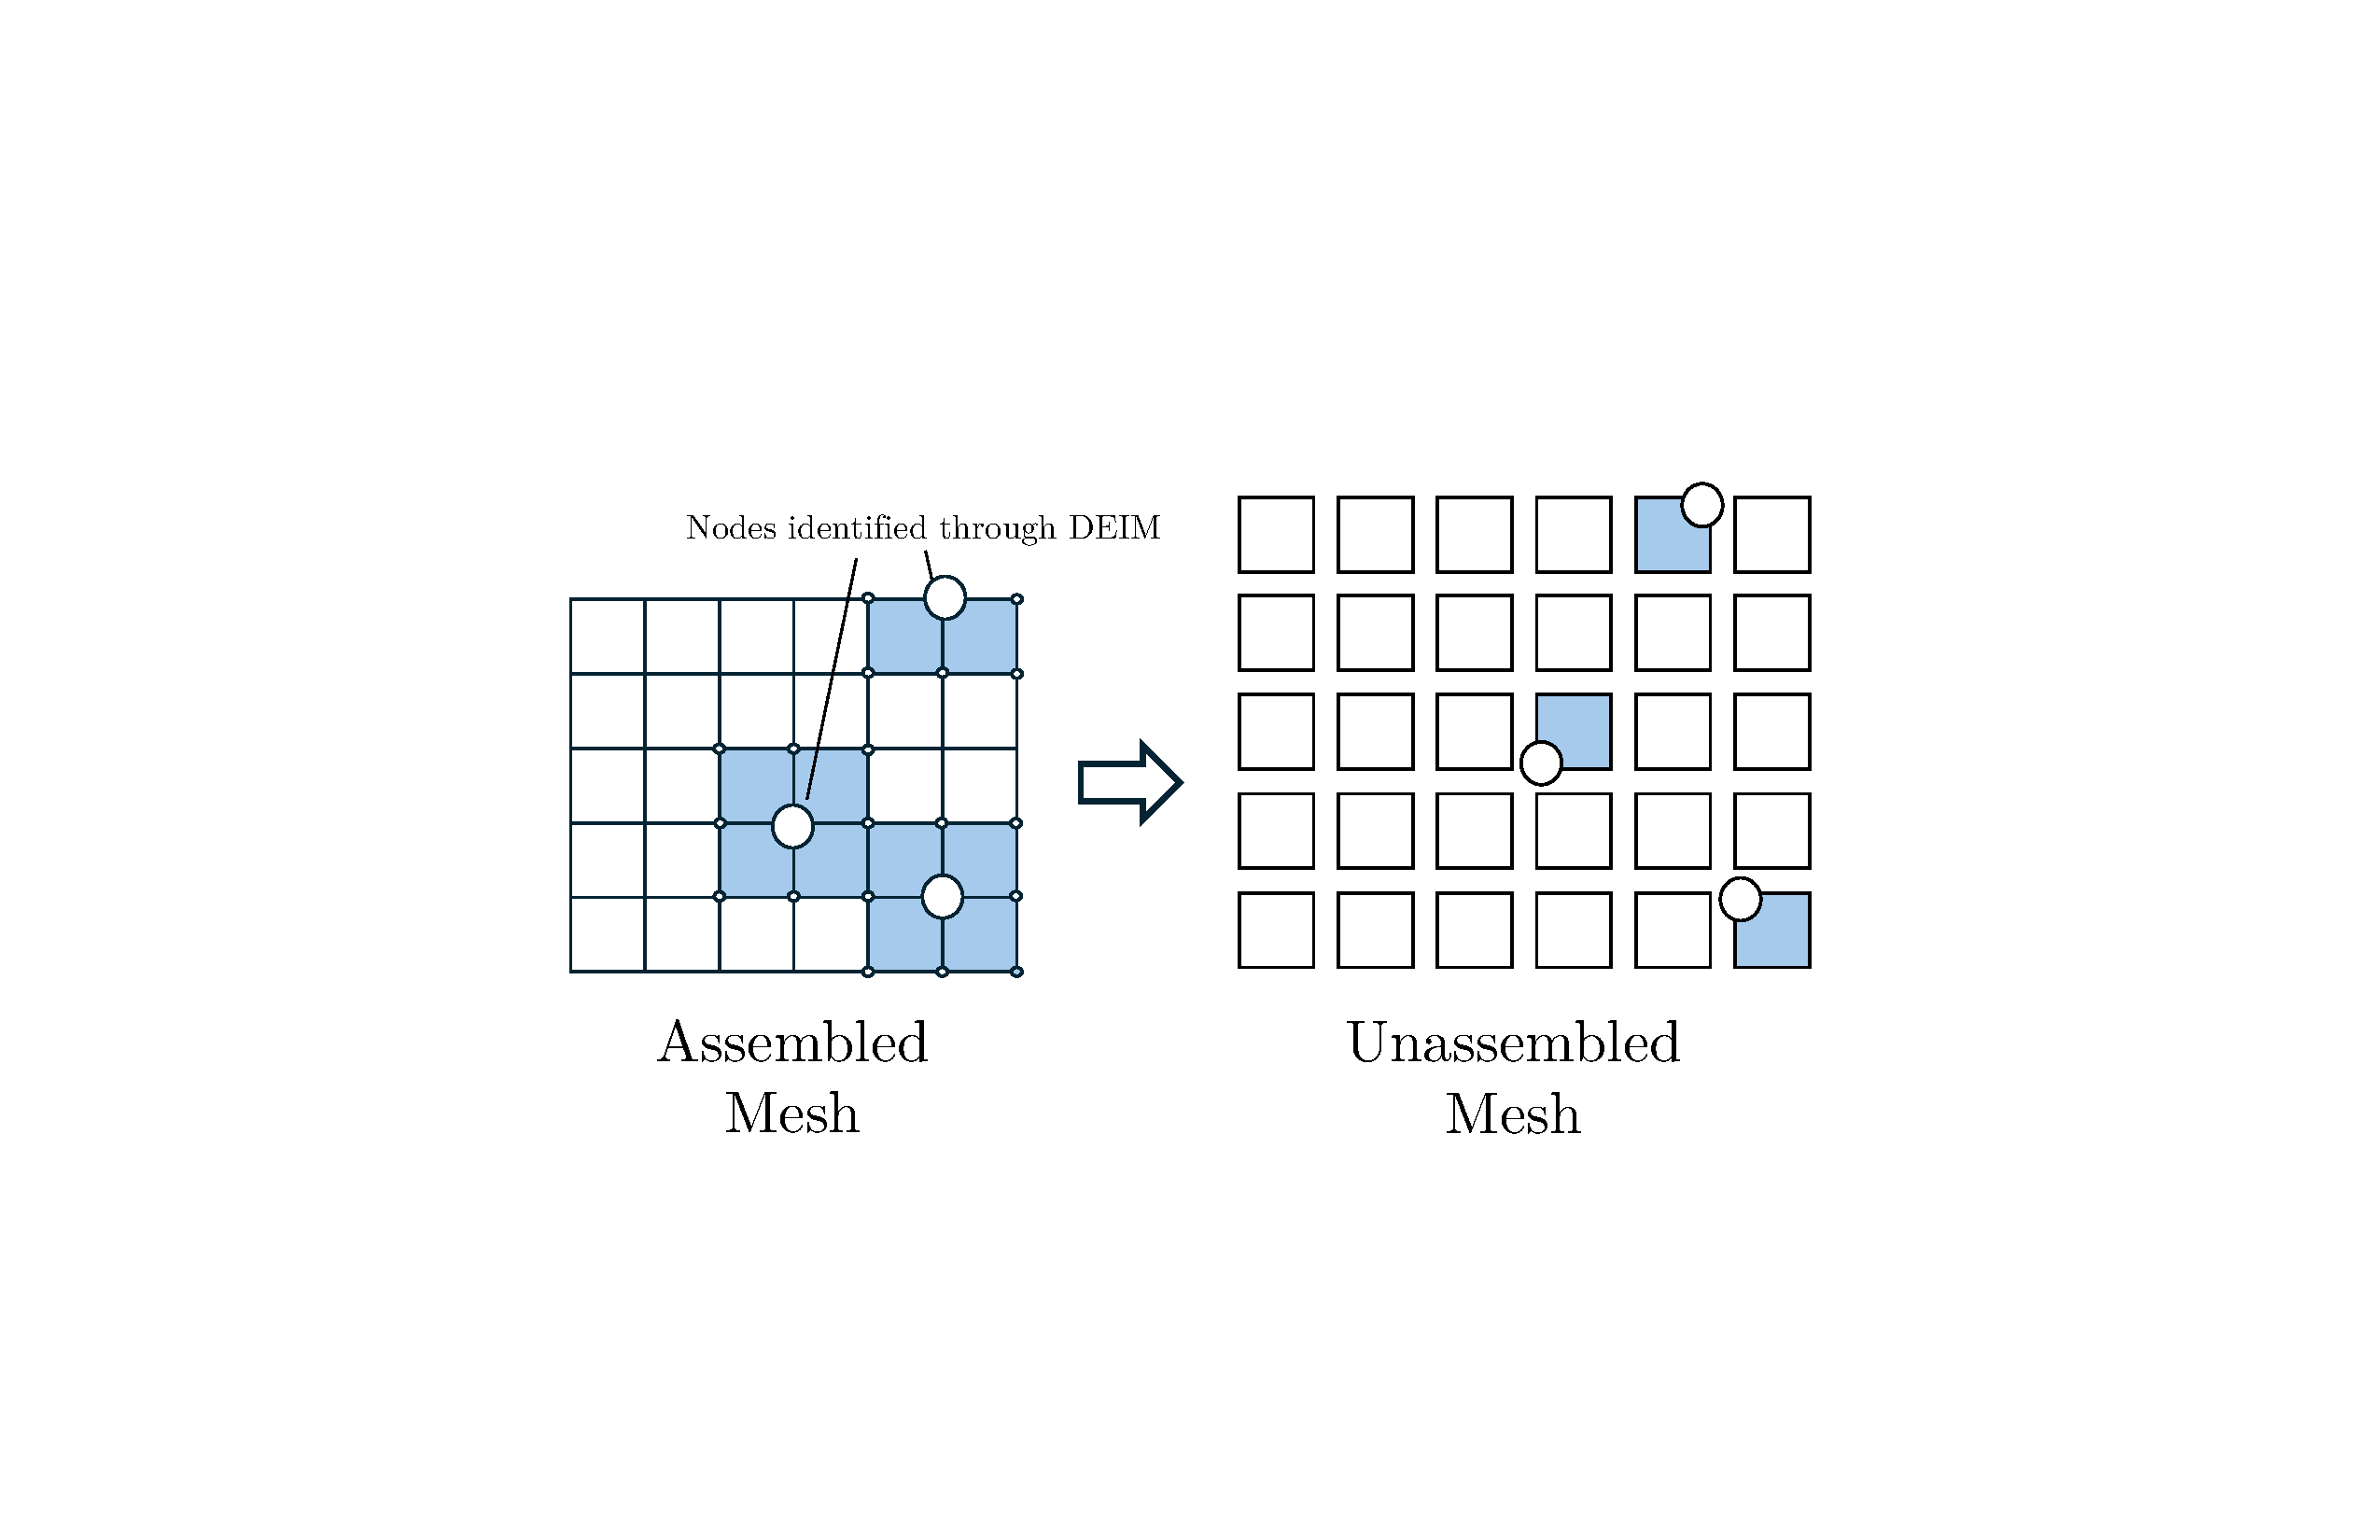
\includegraphics[width=0.7\linewidth]{udeim2.pdf}
    \caption{Unsassembled DEIM requires less elements to be sampled than the traditional DEIM algorithm for Finite Element problems. (Adapted from \cite{tiso2013discrete})}
    \label{fig:UDEIM}
\end{figure}

\begin{figure}
    \centering
    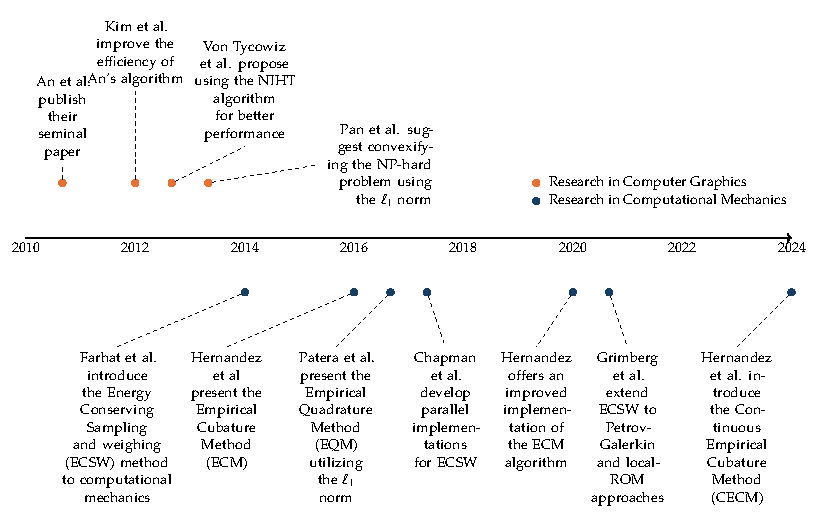
\includegraphics[width=\linewidth]{PAT.pdf}
\caption{A brief history of cubature rules/mesh sampling procedures \cite{an2009optimizing,kim2013subspace,von2013efficient,pan2015subspace,farhat2014dimensional,chapman2016accelerated,Patera_2017_EQP,hernandez2020multiscale,grimberg2021mesh,hernandez2024cecm}. Adapted from \cite{bravo2024subspace}.}
\label{fig:PTA_LIT}
\end{figure}

\begin{figure}[t]
    \centering
    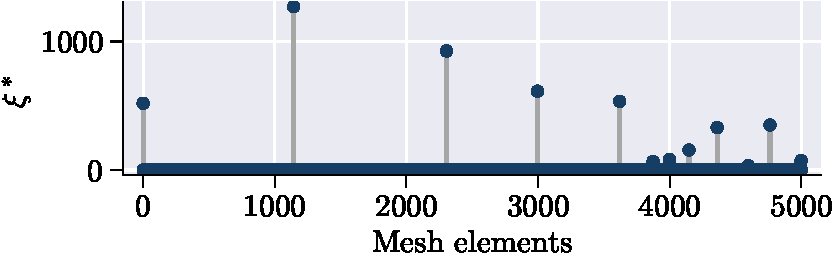
\includegraphics[width=0.8\linewidth]{reduced_mesh_ECSW_new.pdf}
    \caption{Stem plot illustrating the reduced mesh obtained via ECSW-based hyper-reduction. The plot highlights the mesh elements with non-zero weights $\xi^*$ (Eq.~\ref{eq:NNLS}). The weights for all elements lying on the blue line are zero. The reduced mesh comprises only 11 elements, which constitutes 0.2\% of the total 5,000 elements in the original mesh.}
    \label{fig:reduced_mesh_ecsw}
\end{figure}

\begin{figure}[t]
    \centering
    \begin{subfigure}{0.48\linewidth}
        \hspace{-15pt}
        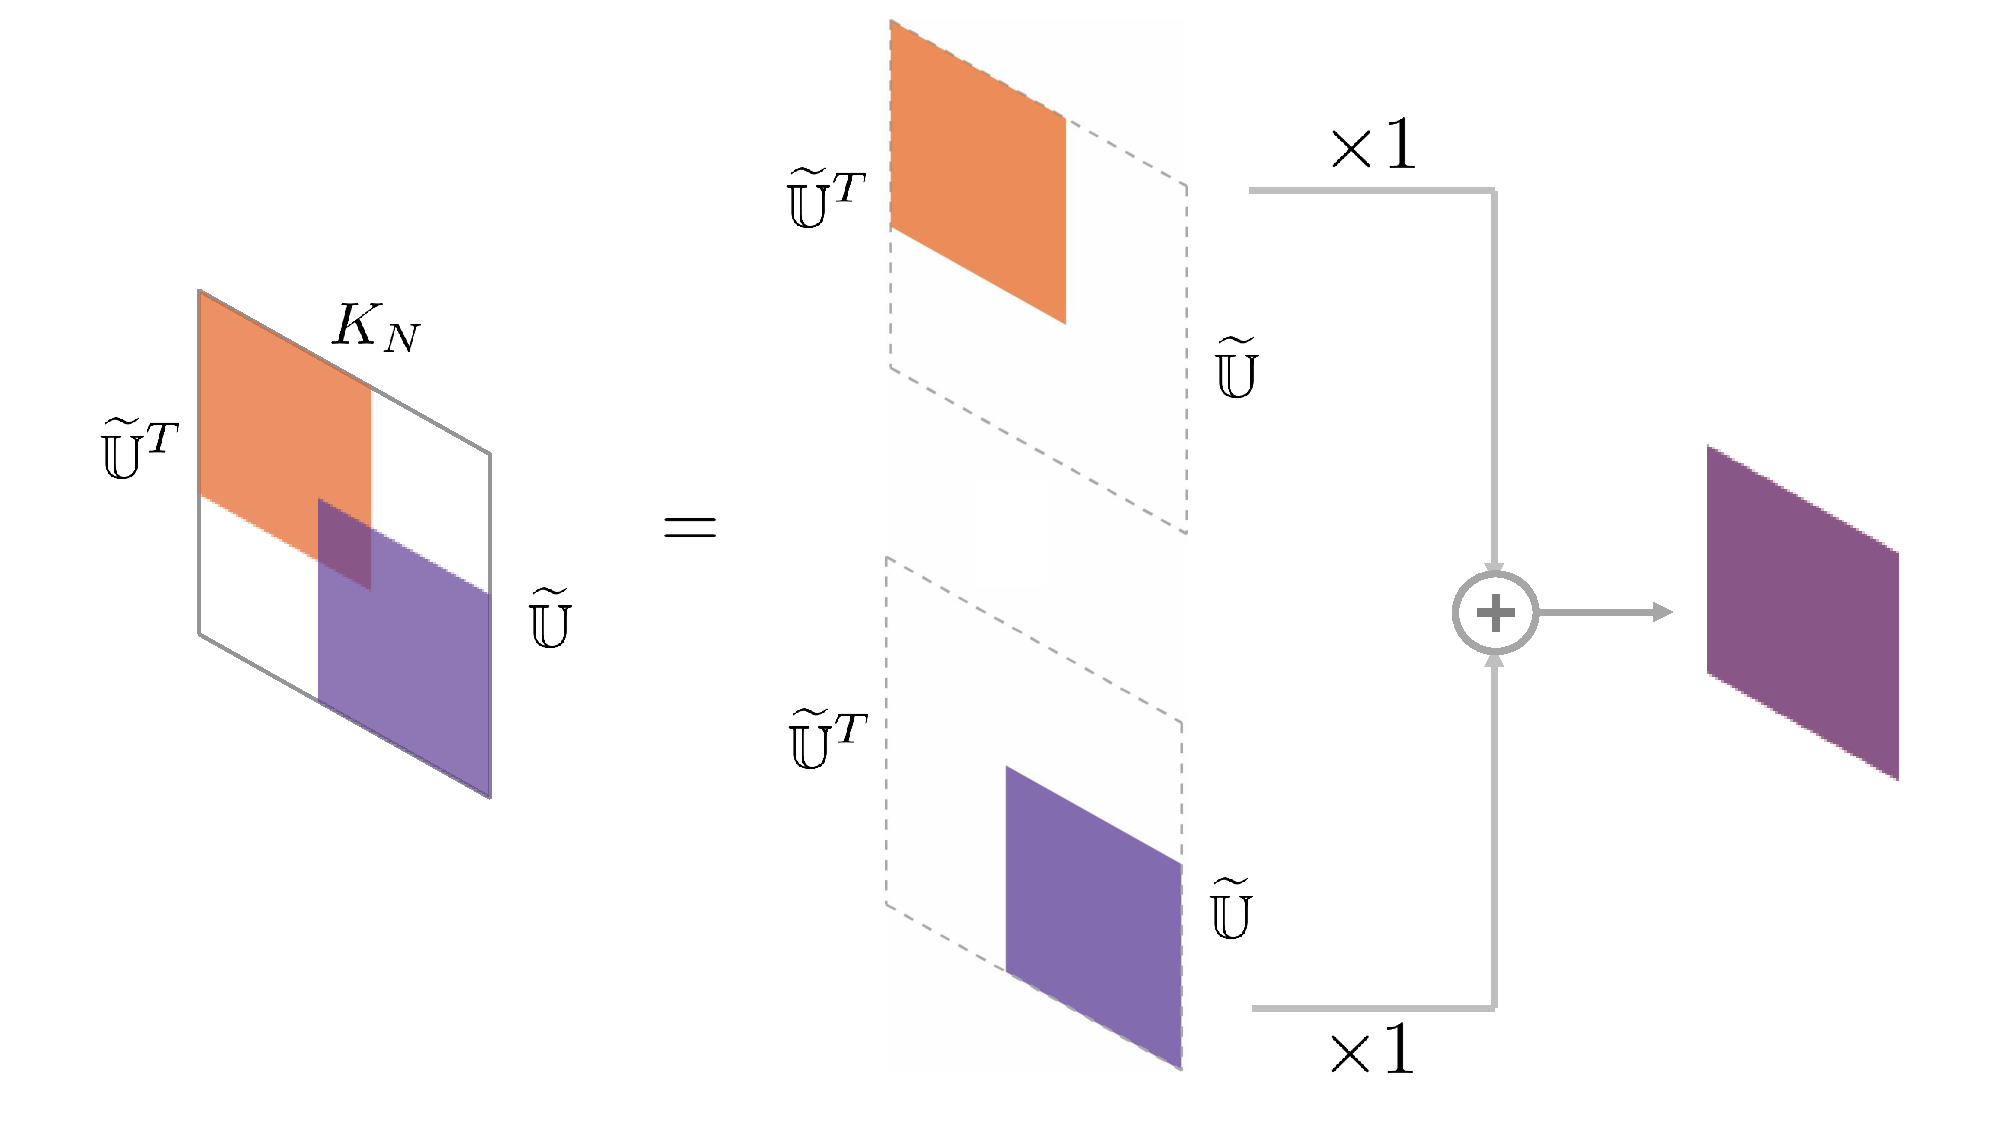
\includegraphics[width=\linewidth]{K_red.pdf}
        \caption{}
        \label{fig:visual_FOM_FEA_2}
    \end{subfigure}%
\begin{subfigure}{0.48\linewidth}
        \centering
        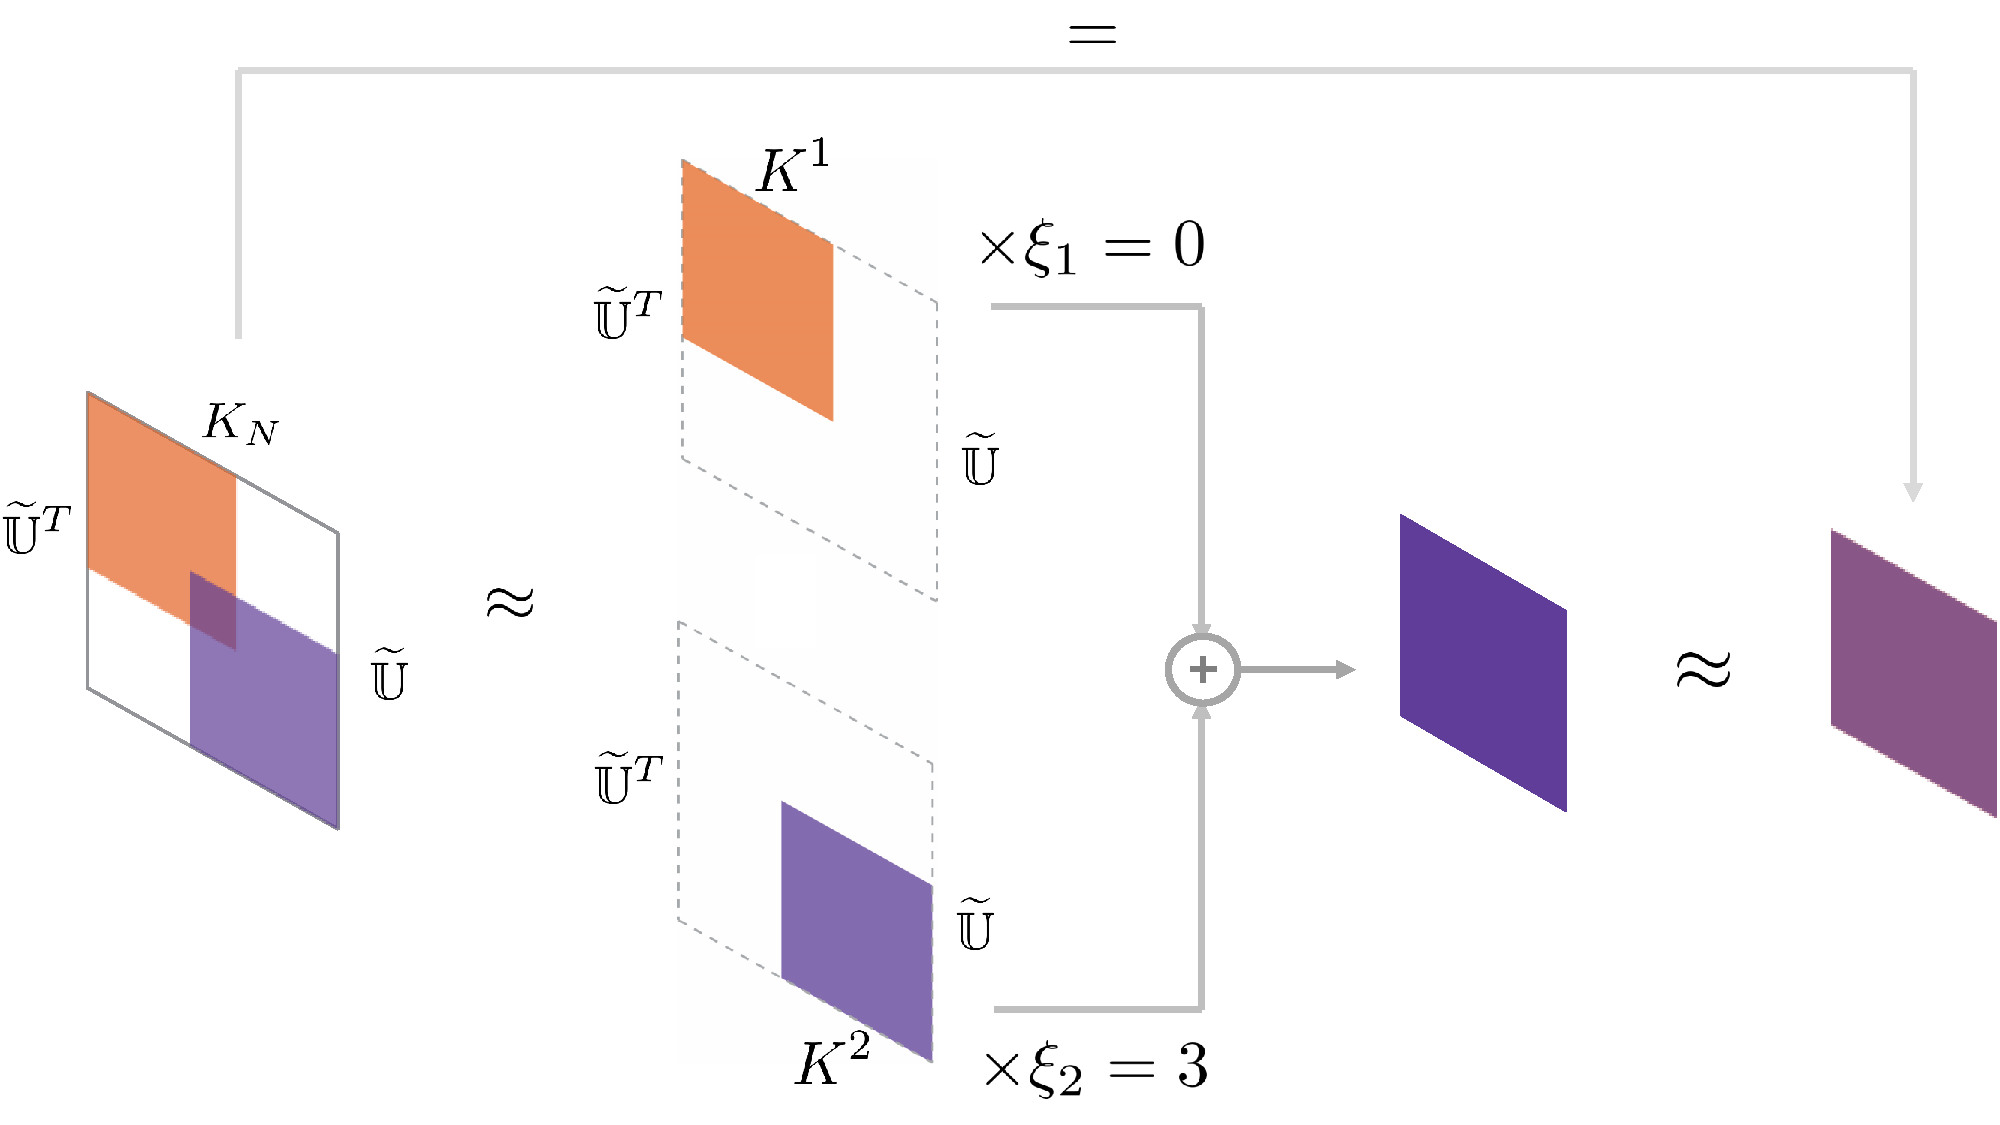
\includegraphics[width=\linewidth]{K_hyper_red.pdf}
        \caption{}
        \label{fig:visual_ROM_FEA}
    \end{subfigure}
\caption{Reduction in the computational cost of evaluating the reduced nonlinear stiffness matrix achieved with ECSW during the iterative solution process. (a) Derivation of the reduced stiffness matrix with equally weighted elemental contributions without hyper-reduction. (b) Efficient \textit{approximation} of the reduced stiffness matrix where the top element's weight \(\xi_1\) is zero, and the bottom element has a much larger weight \(\xi_2\), eliminating the cost of evaluating the top stiffness matrix during solution iteration.}
\label{fig:stiffness_matrices}
\end{figure}

\begin{figure}[t]
\centering
\begin{subfigure}[b]{0.47\linewidth}
\centering
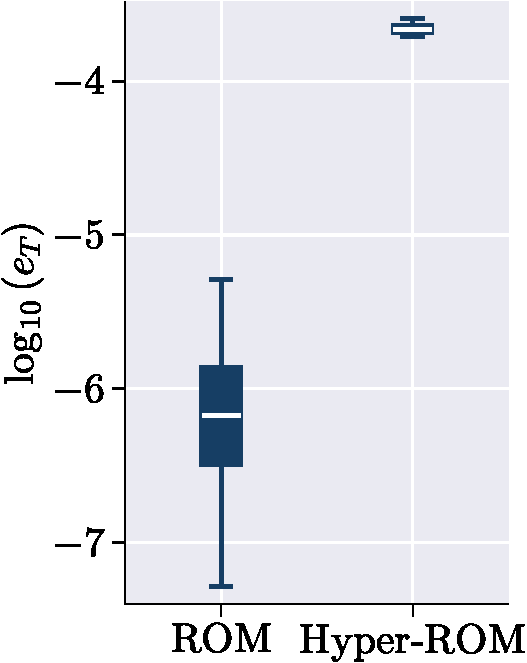
\includegraphics[height=0.95\linewidth]{error_comp_rom_hrom_ecsw.pdf}
\caption{}
\label{fig:HROM_ERROR_SPDUP_a}
\end{subfigure}\hfill
\begin{subfigure}[b]{0.47\linewidth}
\centering
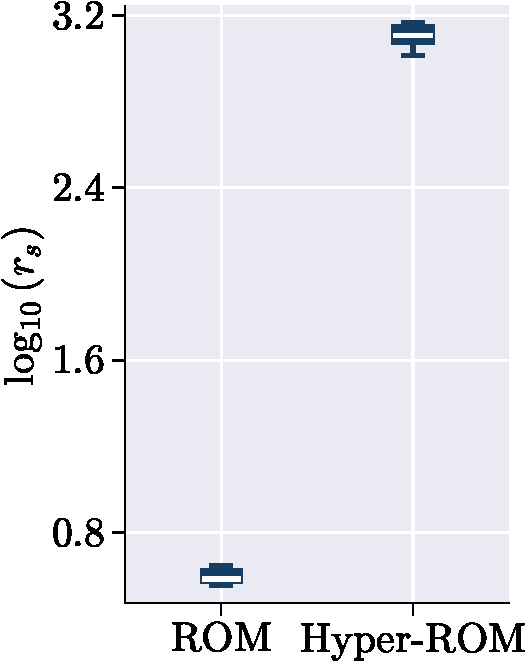
\includegraphics[height=0.95\linewidth]{speed_up_comp_rom_hrom_ecsw.pdf}
\caption{}
\label{fig:HROM_ERROR_SPDUP_b}
\end{subfigure}
\caption{Difference in accuracy ($e_T$) and speed-up ($r_s$) between the regular projection based ROM and ECSW Hyper-ROM.}
\label{fig:HROM_ERROR_SPDUP}
\end{figure}

\begin{figure}[t]
    \centering
    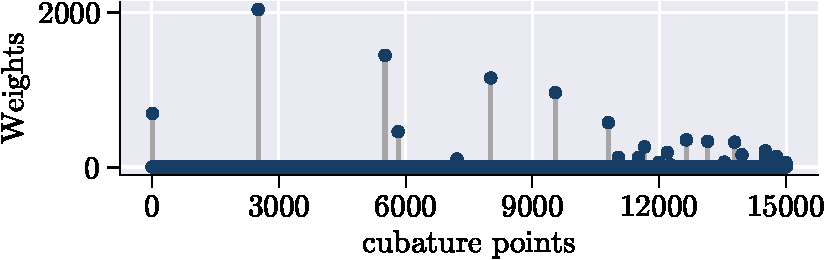
\includegraphics[width=0.8\linewidth]{reduced_mesh_empCM.pdf}
    \caption{Sparse distribution of cubature points and corresponding weights achieved using the ECM-based hyper-reduction technique. The ECM algorithm selected 30 points out of 15,000 cubature points (3 cubature points/element) employed in the high-fidelity model. The resulting reduced mesh effectively contains 26 elements out of 5,000 in the high-fidelity model, accounting for approximately 0.52\% of the total elements in the original mesh.}
    \label{fig:reduced_mesh_ecm}
\end{figure}

\begin{figure}[t!]
\centering
\begin{subfigure}[b]{0.33\linewidth}
\centering
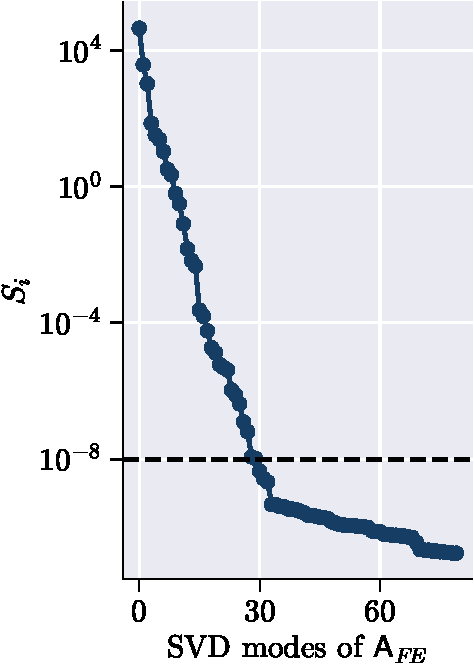
\includegraphics[height=1.3\linewidth]{S_AFE.pdf}
\caption{}
\label{fig:svd_AE}
\end{subfigure}\hfill
\begin{subfigure}[b]{0.33\linewidth}
\centering
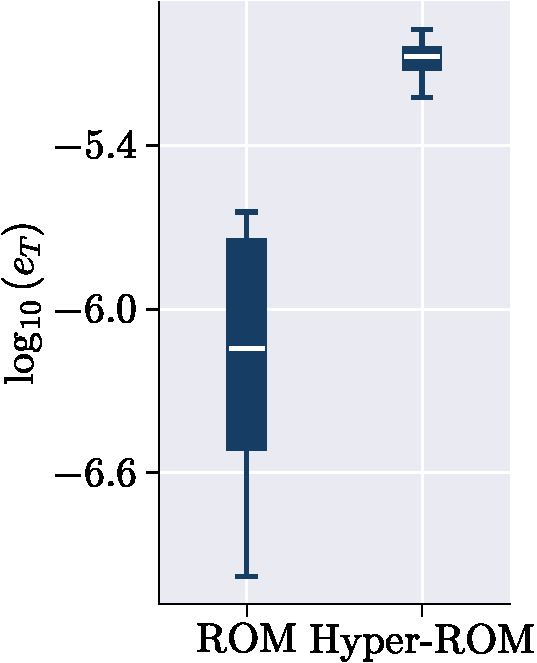
\includegraphics[height=1.3\linewidth]{error_comp_rom_hrom_ecm.pdf}
\caption{}
\label{fig:HROM_ERROR_SPDUP__ecm_a}
\end{subfigure}
\begin{subfigure}[b]{0.33\linewidth}
\centering
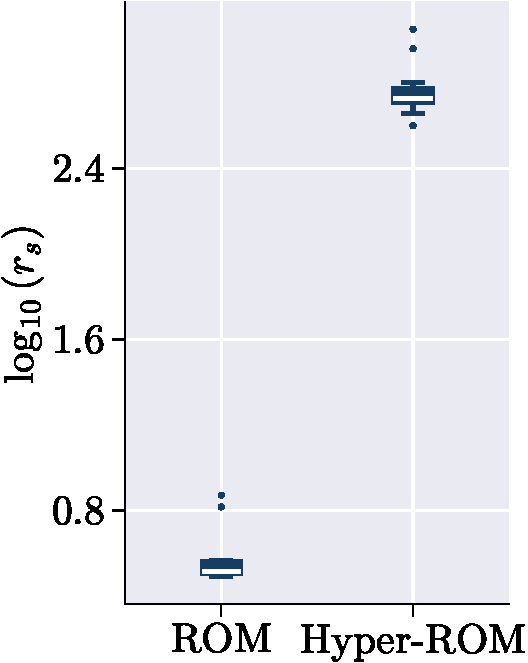
\includegraphics[height=1.3\linewidth]{speed_up_comp_rom_hrom_ecm.pdf}
\caption{}
\label{fig:HROM_ERROR_SPDUP__ecm_b}
\end{subfigure}
\caption{(a) Decay of the singular values of the ECM matrix \(\mat{A}_{FE}\), which is compressed to enhance computational efficiency in identifying a sparse set of cubature points. (b) Difference in accuracy (\(e_T\)) and (c) speed-up (\(r_s\)) between the regular projection-based ROM and the ECM Hyper-ROM.}
\label{fig:HROM_ERROR_SPDUP_ecm}
\end{figure}

\begin{figure}[t]
    \centering
    \begin{subfigure}[b]{0.35\linewidth}
    \centering
    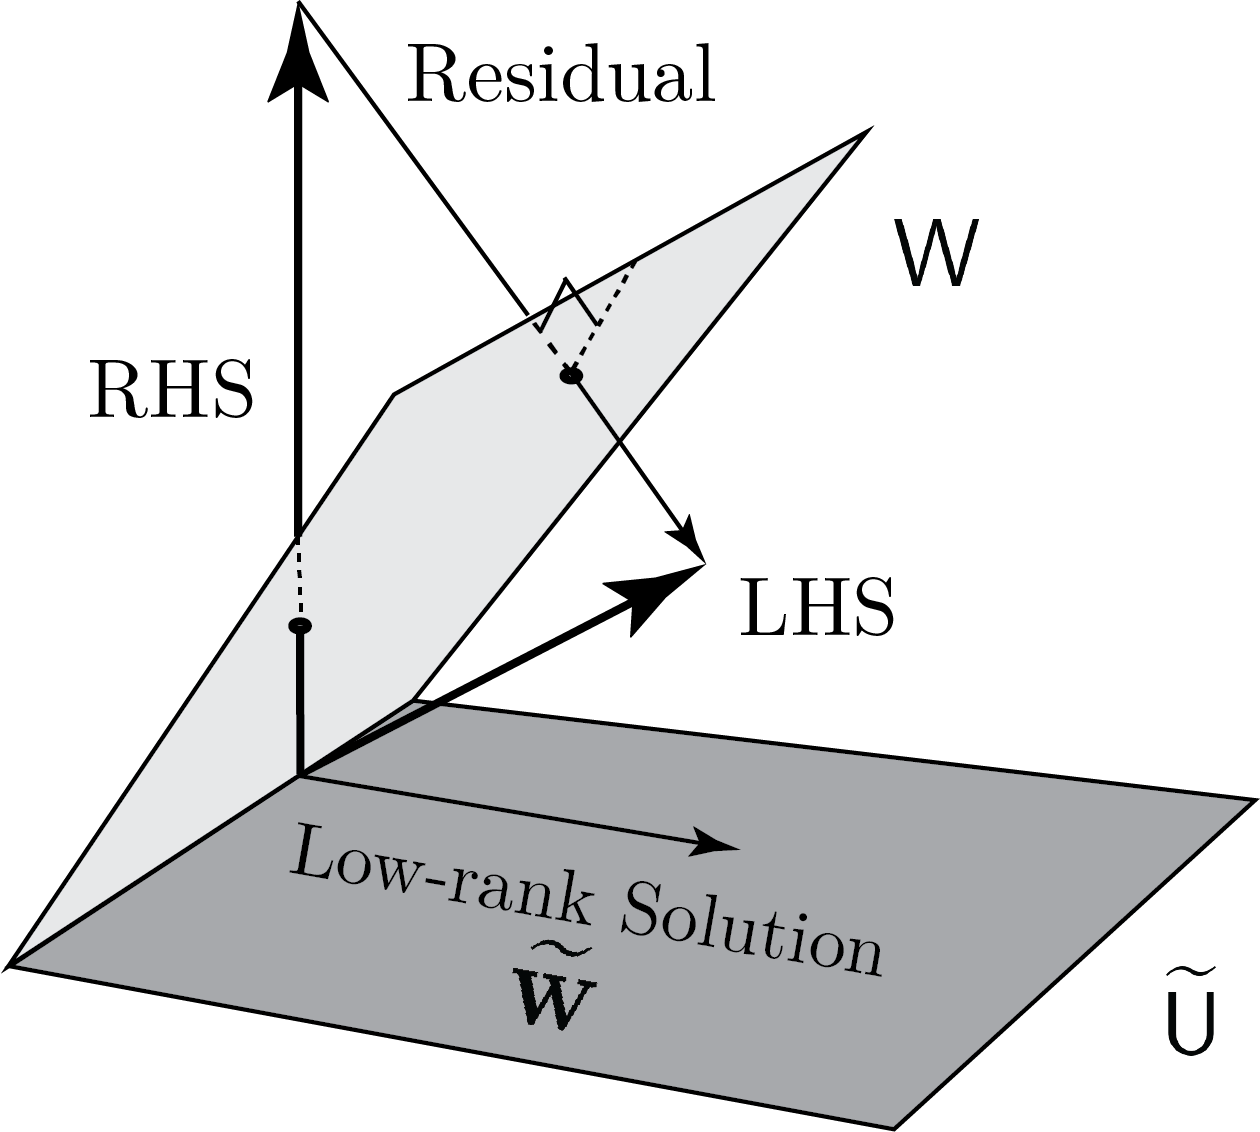
\includegraphics[width=\linewidth]{PG.png}
    \caption{}
    \label{fig:projections_PG}
    \end{subfigure}\hfill
    \begin{subfigure}[b]{0.35\linewidth}
    \centering
    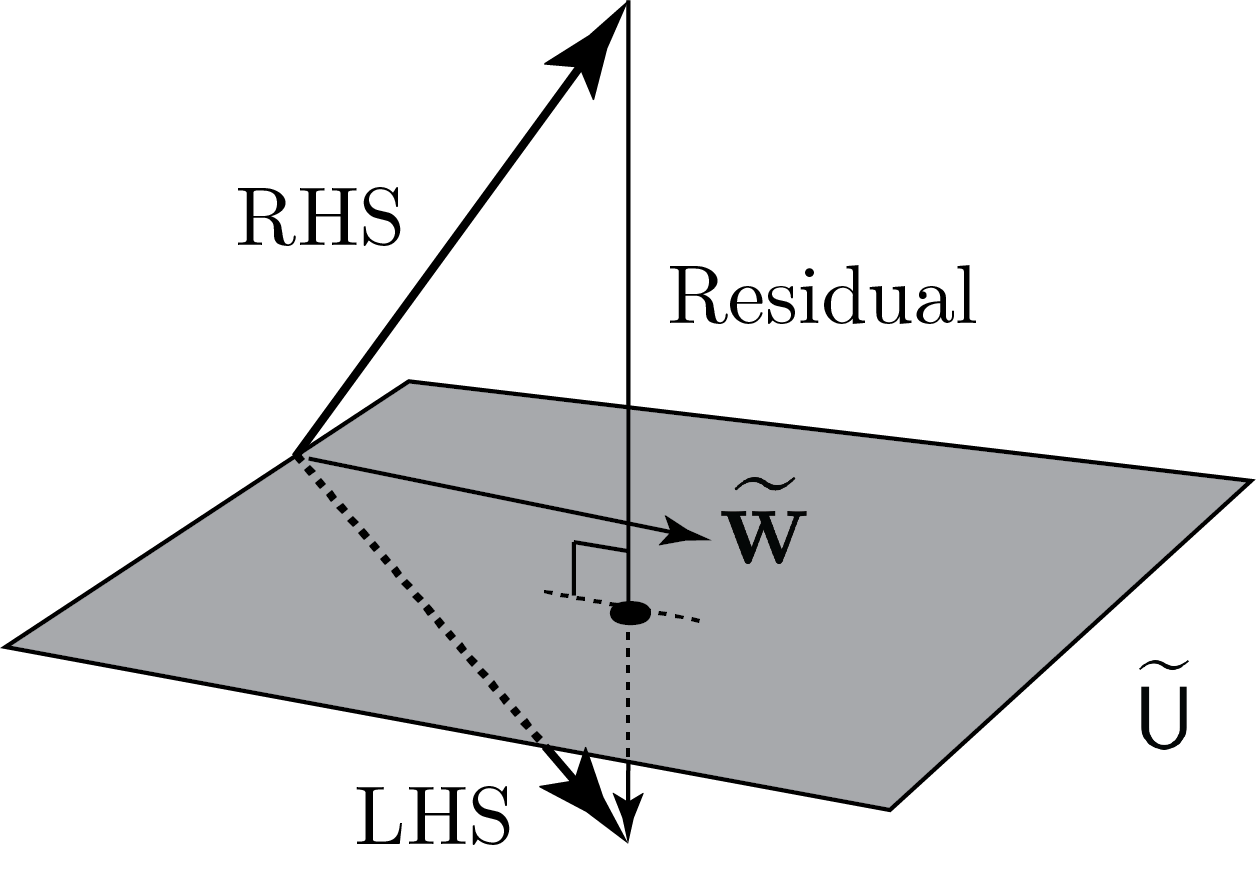
\includegraphics[width=\linewidth]{G.png}
    \caption{}
    \label{fig:projections_G}
    \end{subfigure}
    \caption{(a) Petrov-Galerkin Projection (b) Galerkin Projection}
    \label{fig:projections}
    \end{figure}

\end{document}